\documentclass[text.tex]{subfiles}

\begin{document}
In this chapter we demonstrate results that can be obtained using the methods described in previous chapter. 

For each Pisot-cyclotomic number we first show the number itself, several of its properties, then results of analysis of one dimensional quasicrystal.

Results for one dimensional quasicrystal entail table listing the set of distance between consecutive points of the quasicrystal for a window of certain size and two diagrams listing all possible Voronoi tiles and their periods. 

For two dimensions we demonstrate our method with octagonal window and Pisot-cyclotomic number $\beta_8 = 1+\sqrt{2}$. Due to constraints unrelated to our method (insufficient RAM), we were unable to finish the analysis for circular window and $12$-fold rotational symmetry in time. 

Results for the two dimensional quasicrystal were acquired following the following methodology:
\begin{enumerate}
\item acquire the list of Voronoi tiles for quasicrystal with window size $\beta$
\item calculate $\omega_1$ for each Voronoi tile from the list, add each $\omega_1\in(1,\beta]$ to list \texttt{singular}
\item acquire the list of Voronoi tiles for each quasicrystal with window size on the list \texttt{singular}
\item repeat two previous steps until the list \texttt{singular} no longer grows
\item acquire the list of Voronoi tiles for each quasicrystal with window size as mean of two consecutive values on the list \texttt{singular}
\end{enumerate}

Since paper lacks convenient features such as pan and zoom we decided to not print all of the diagrams that show our results. For all diagrams we have acquired please download the package at:\\
\resizebox{\textwidth}{!}{\url{https://github.com/edasubert/quasicrystal/blob/master/RESULTS/results_for_octagonal_window.pdf}}
\resizebox{\textwidth}{!}{\url{https://github.com/edasubert/quasicrystal/blob/master/RESULTS/results_for_circular_window.pdf}}

There you will find two PDFs, one showing the results for octagonal window and second showing work in progress on quasicrystals with $8$-fold rotational symmetry with circular windows. Both PDFs contain division of window, list of Voronoi tiles and a finite sections of the quasicrystal for each window size. 

Further we only show the lists of Voronoi tiles for the octagonal window and estimates of their periods. Since each Voronoi tile may appear in up to $16$ or $24$ possible orientations (rotation and reflection) we only show one representative to conserve space.

\begin{figure}[h!]
\centering
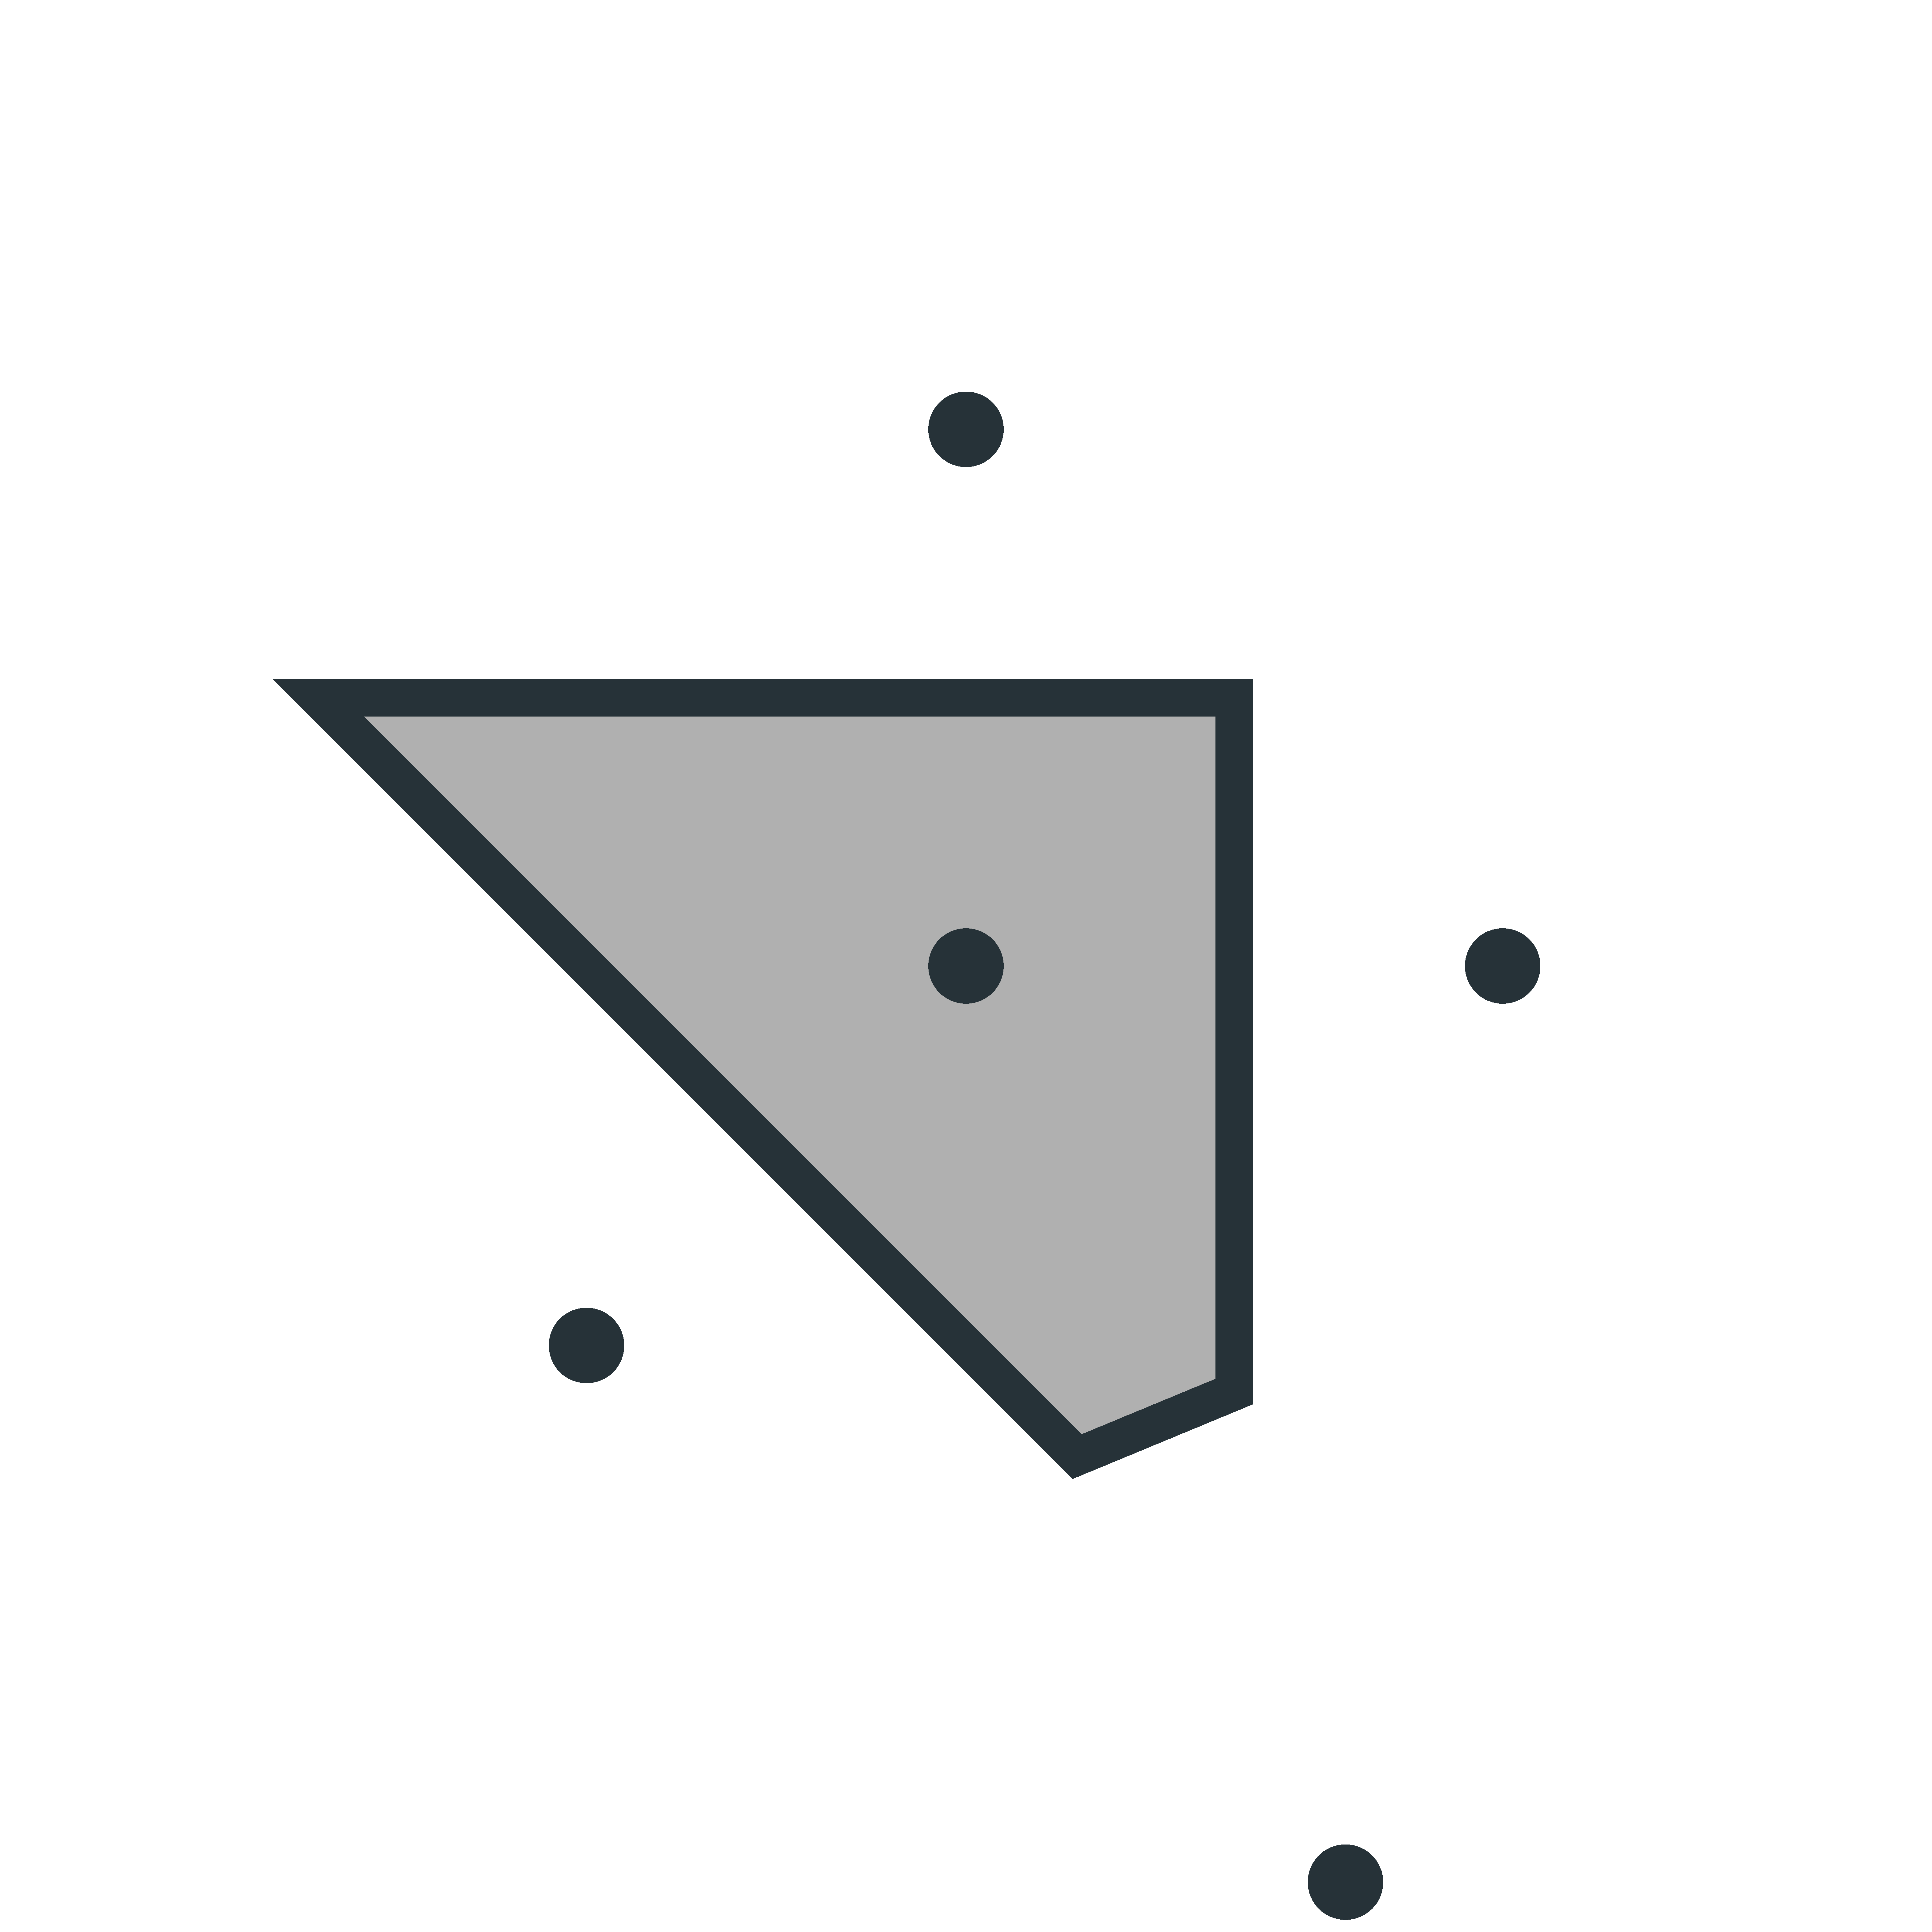
\includegraphics[width=0.11\textwidth]{img/results/tiles/octagon_100000_(1_0alpha_1)_017.pdf}
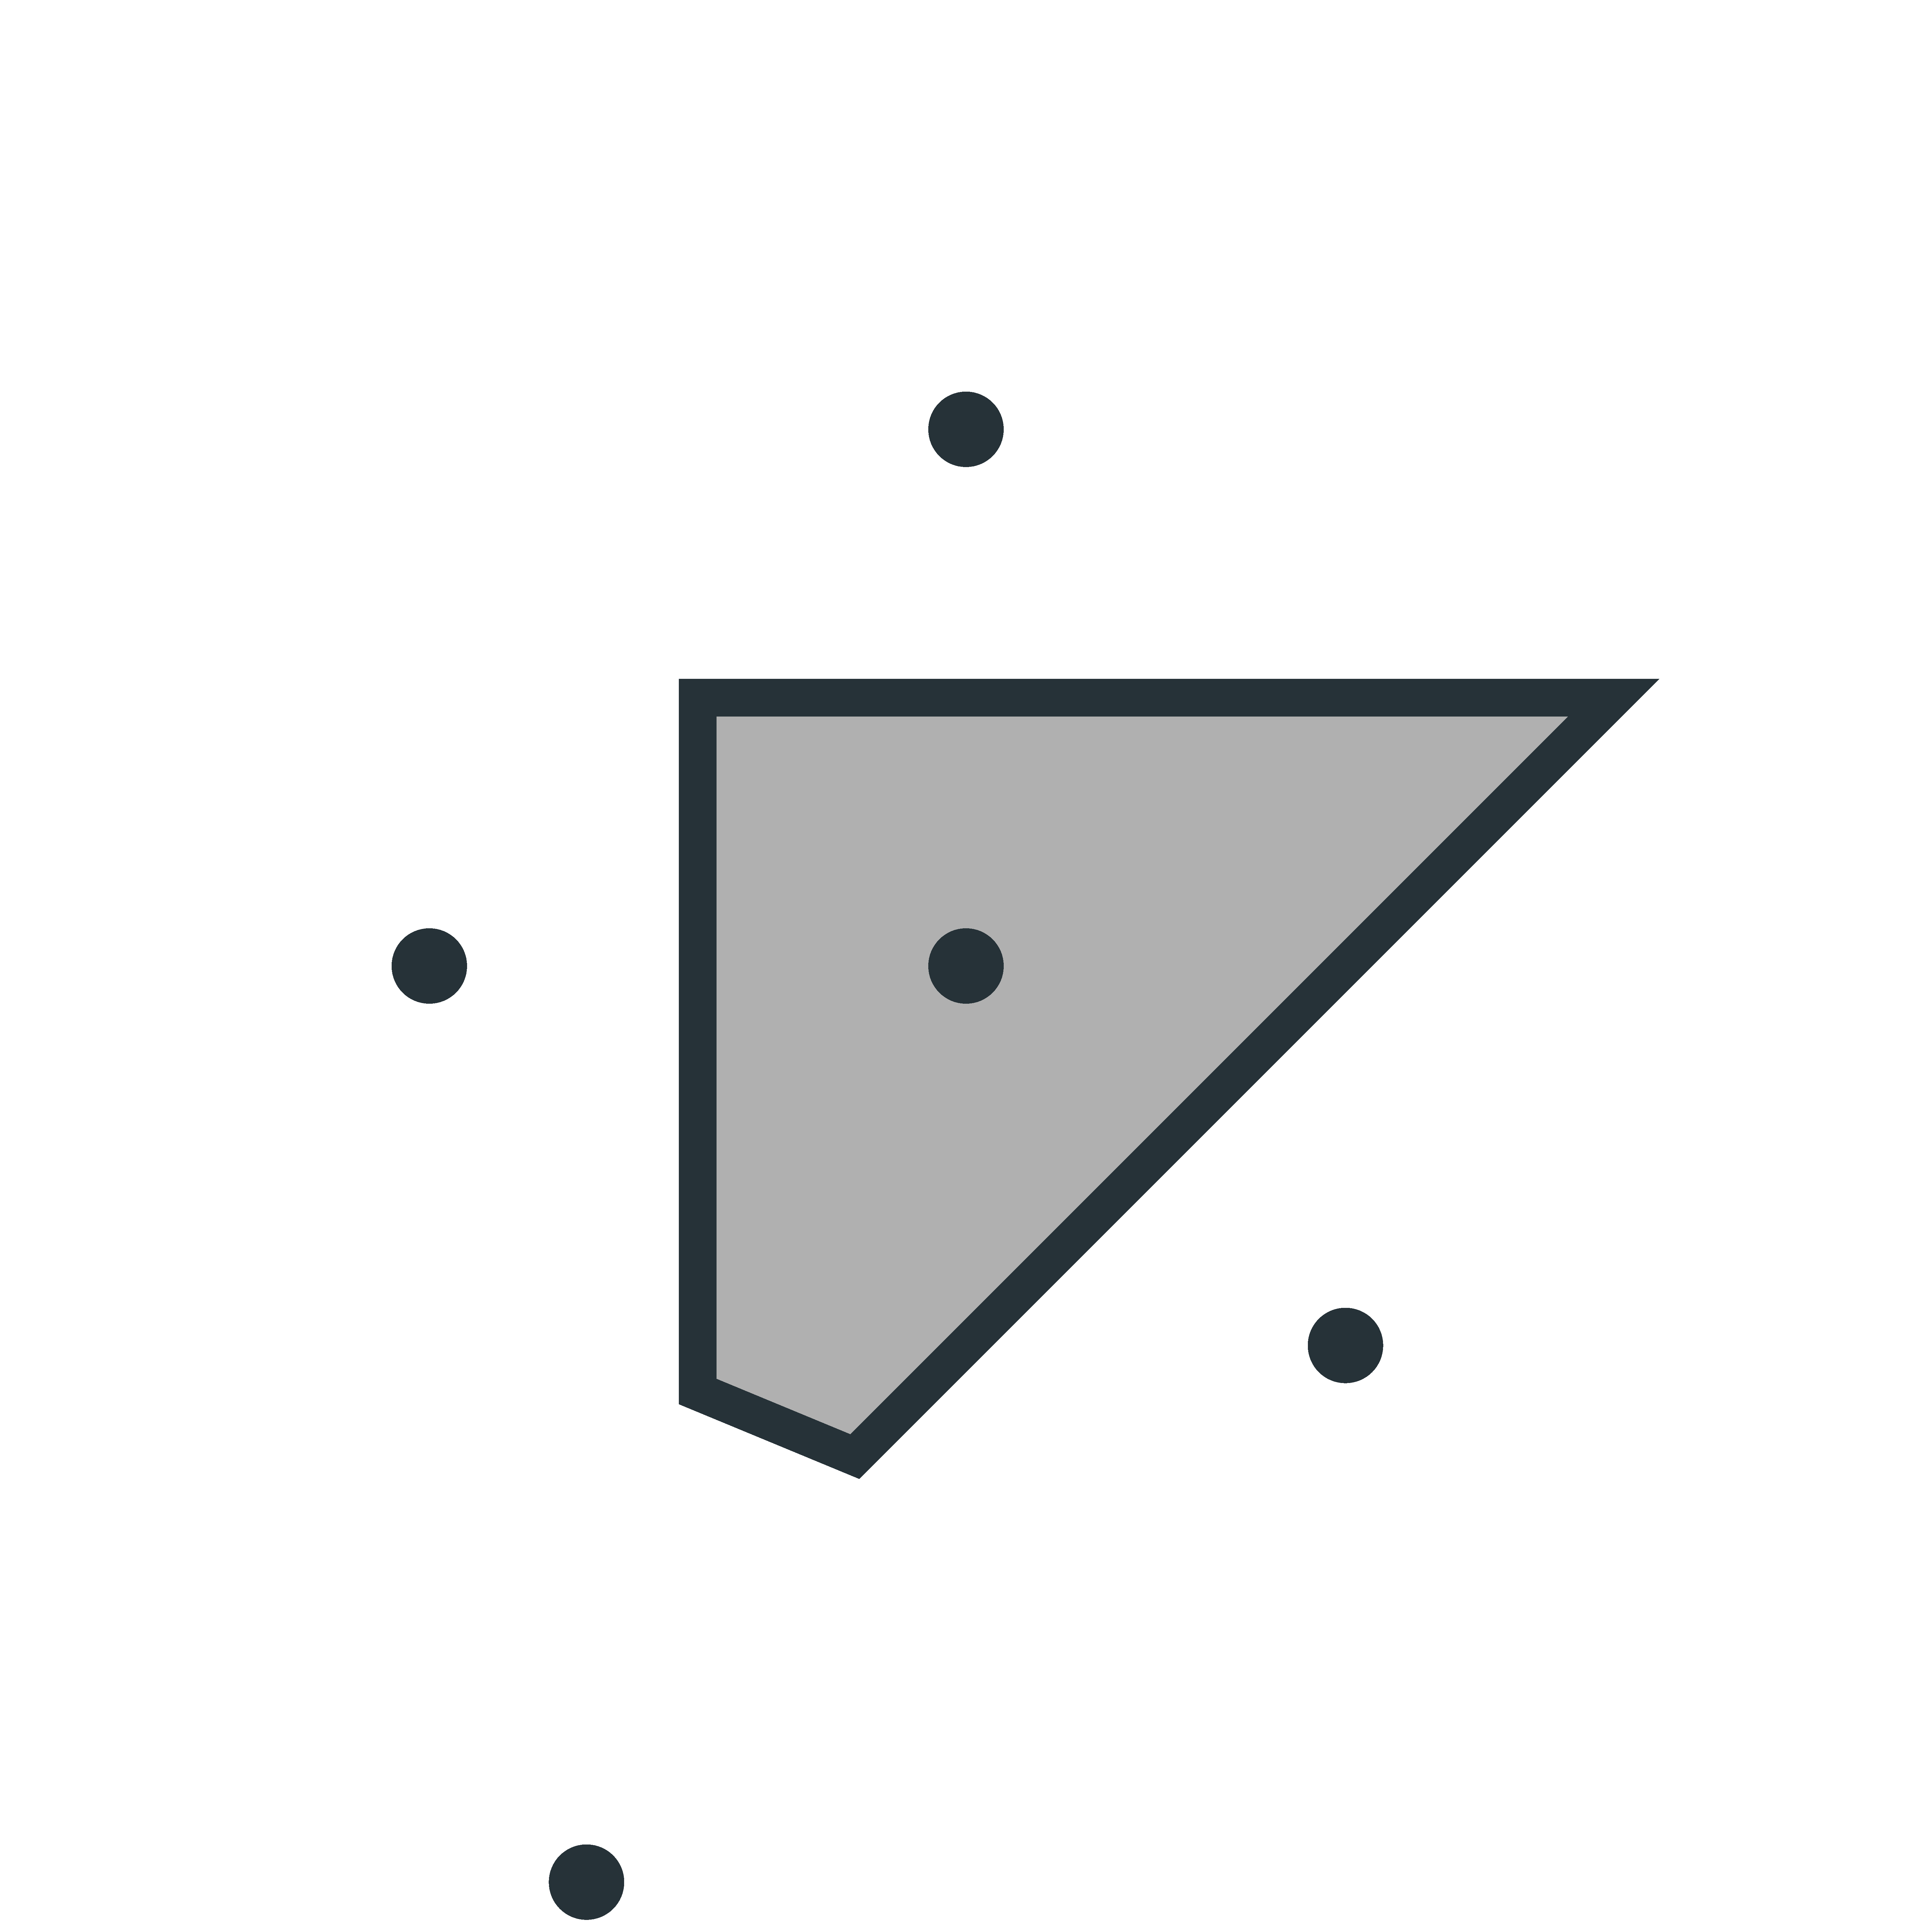
\includegraphics[width=0.11\textwidth]{img/results/tiles/octagon_100000_(1_0alpha_1)_018.pdf}
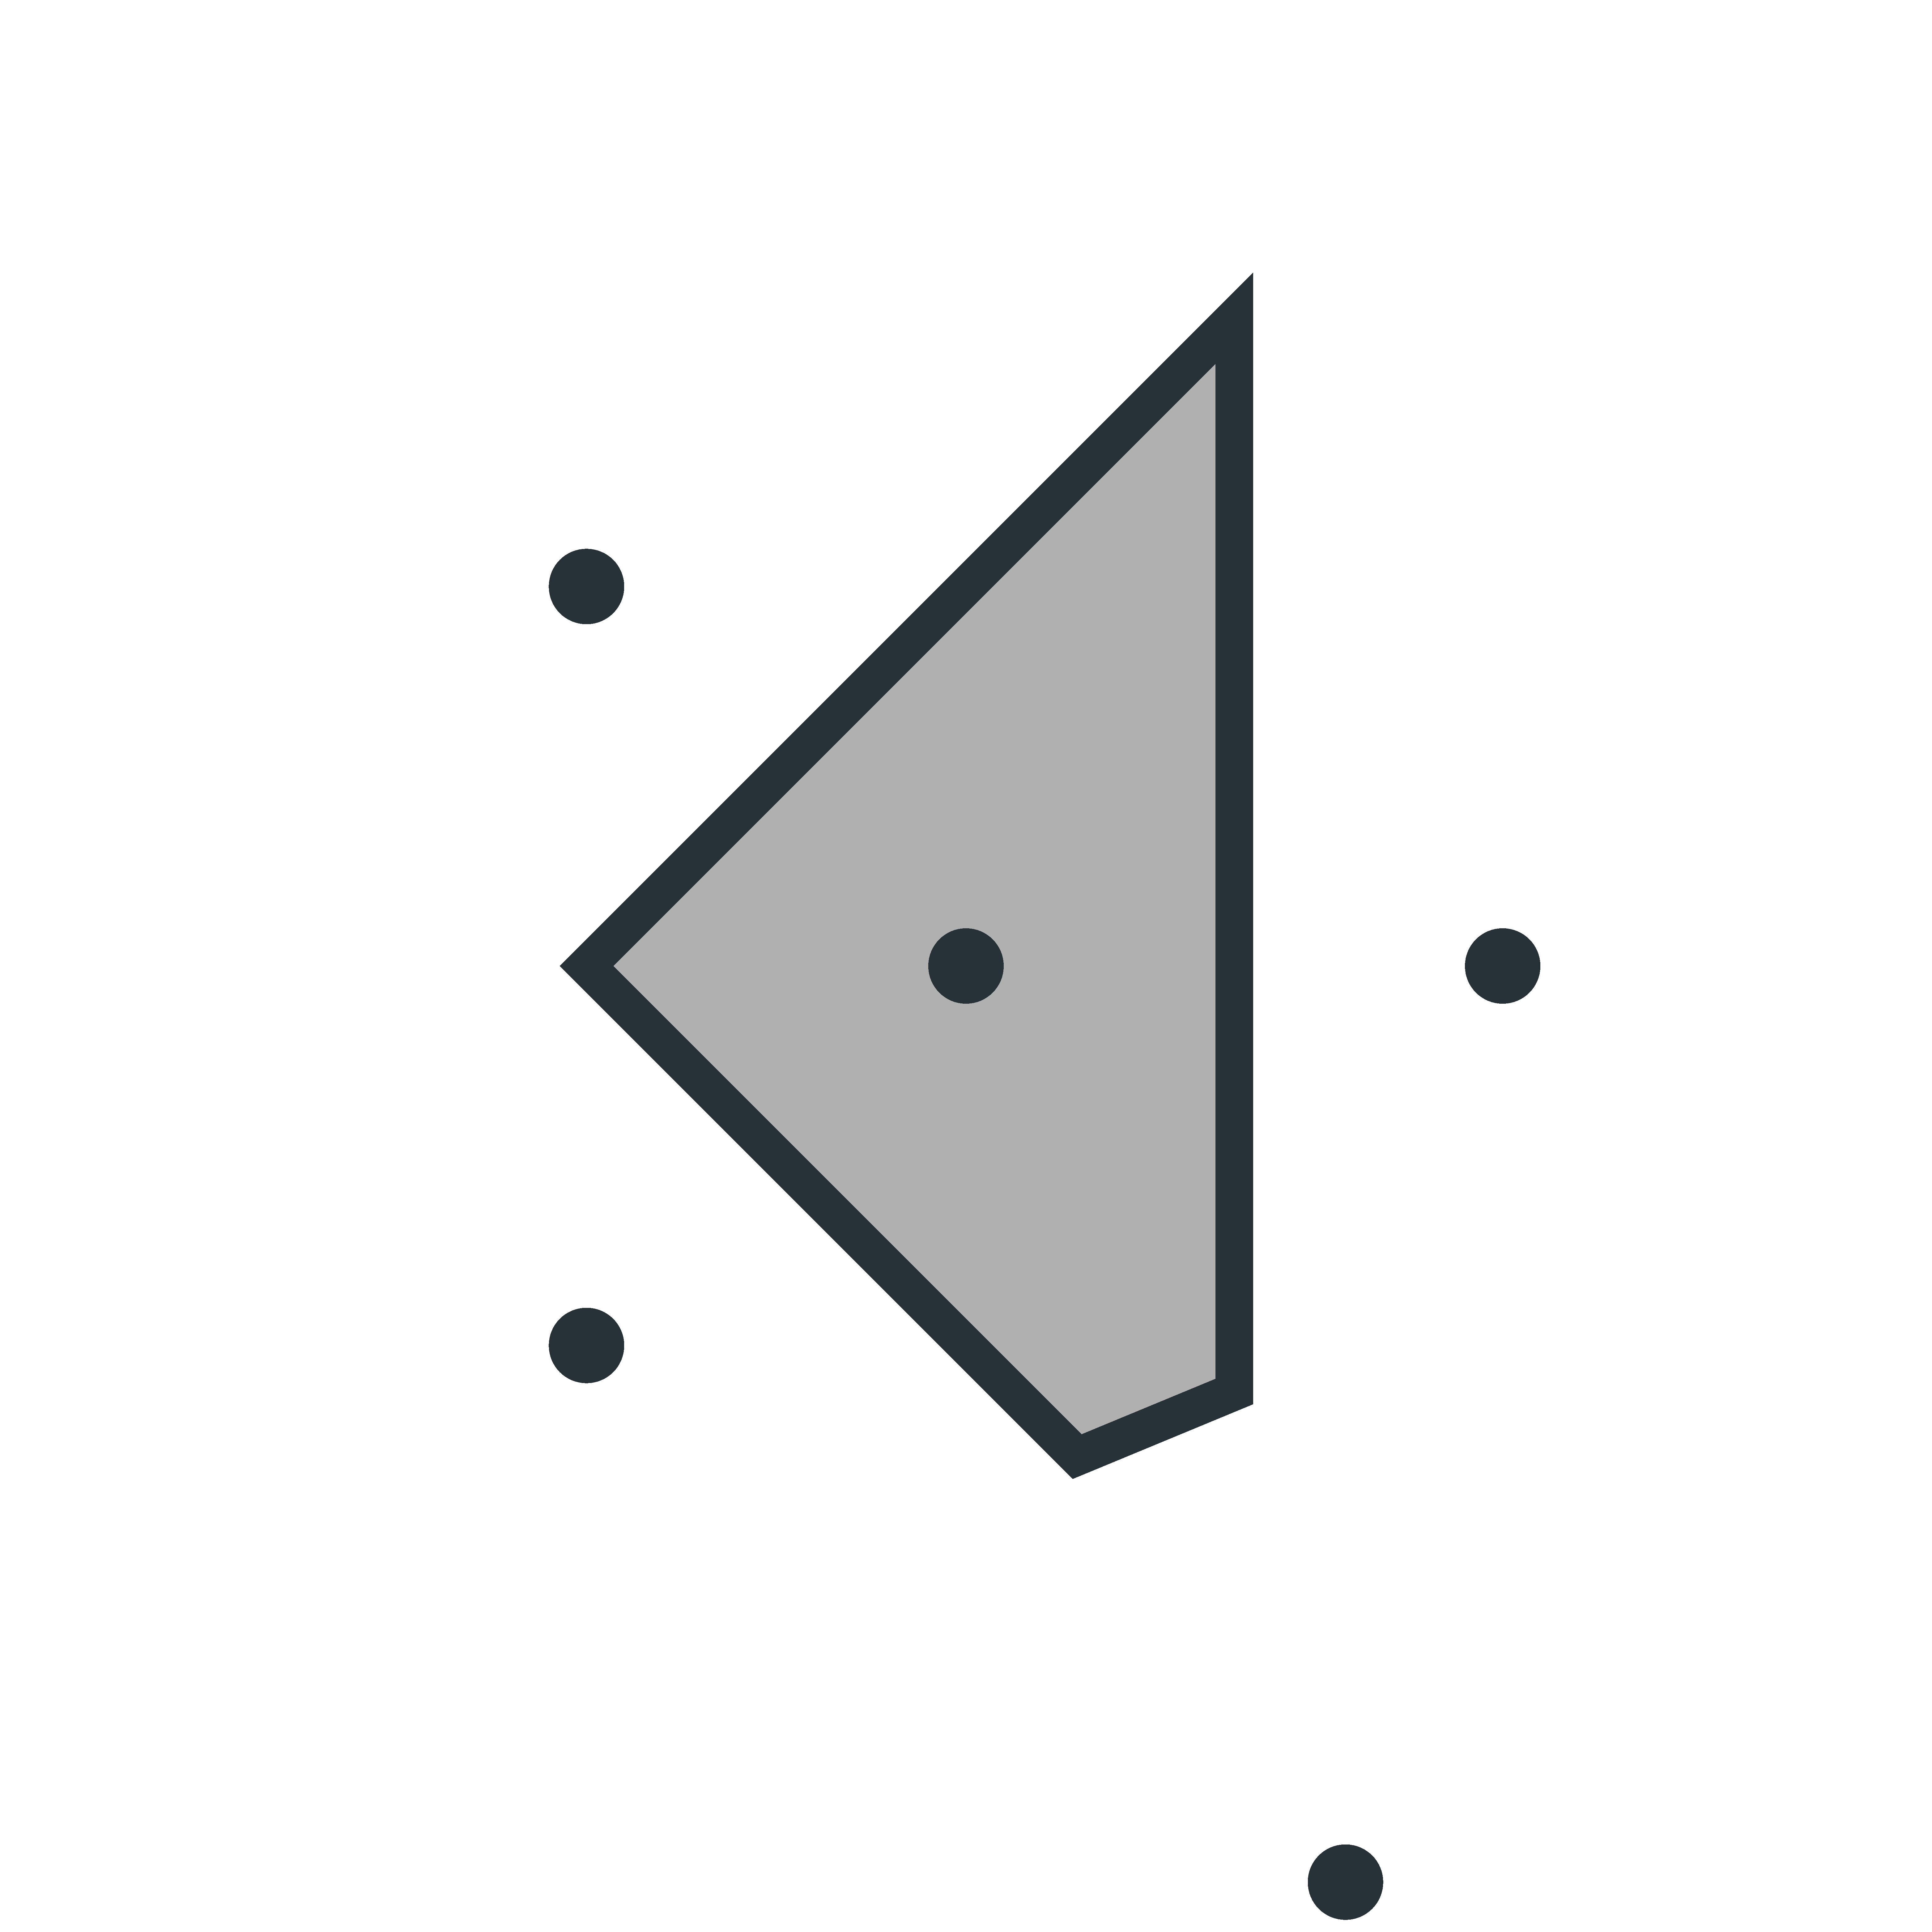
\includegraphics[width=0.11\textwidth]{img/results/tiles/octagon_100000_(1_0alpha_1)_019.pdf}
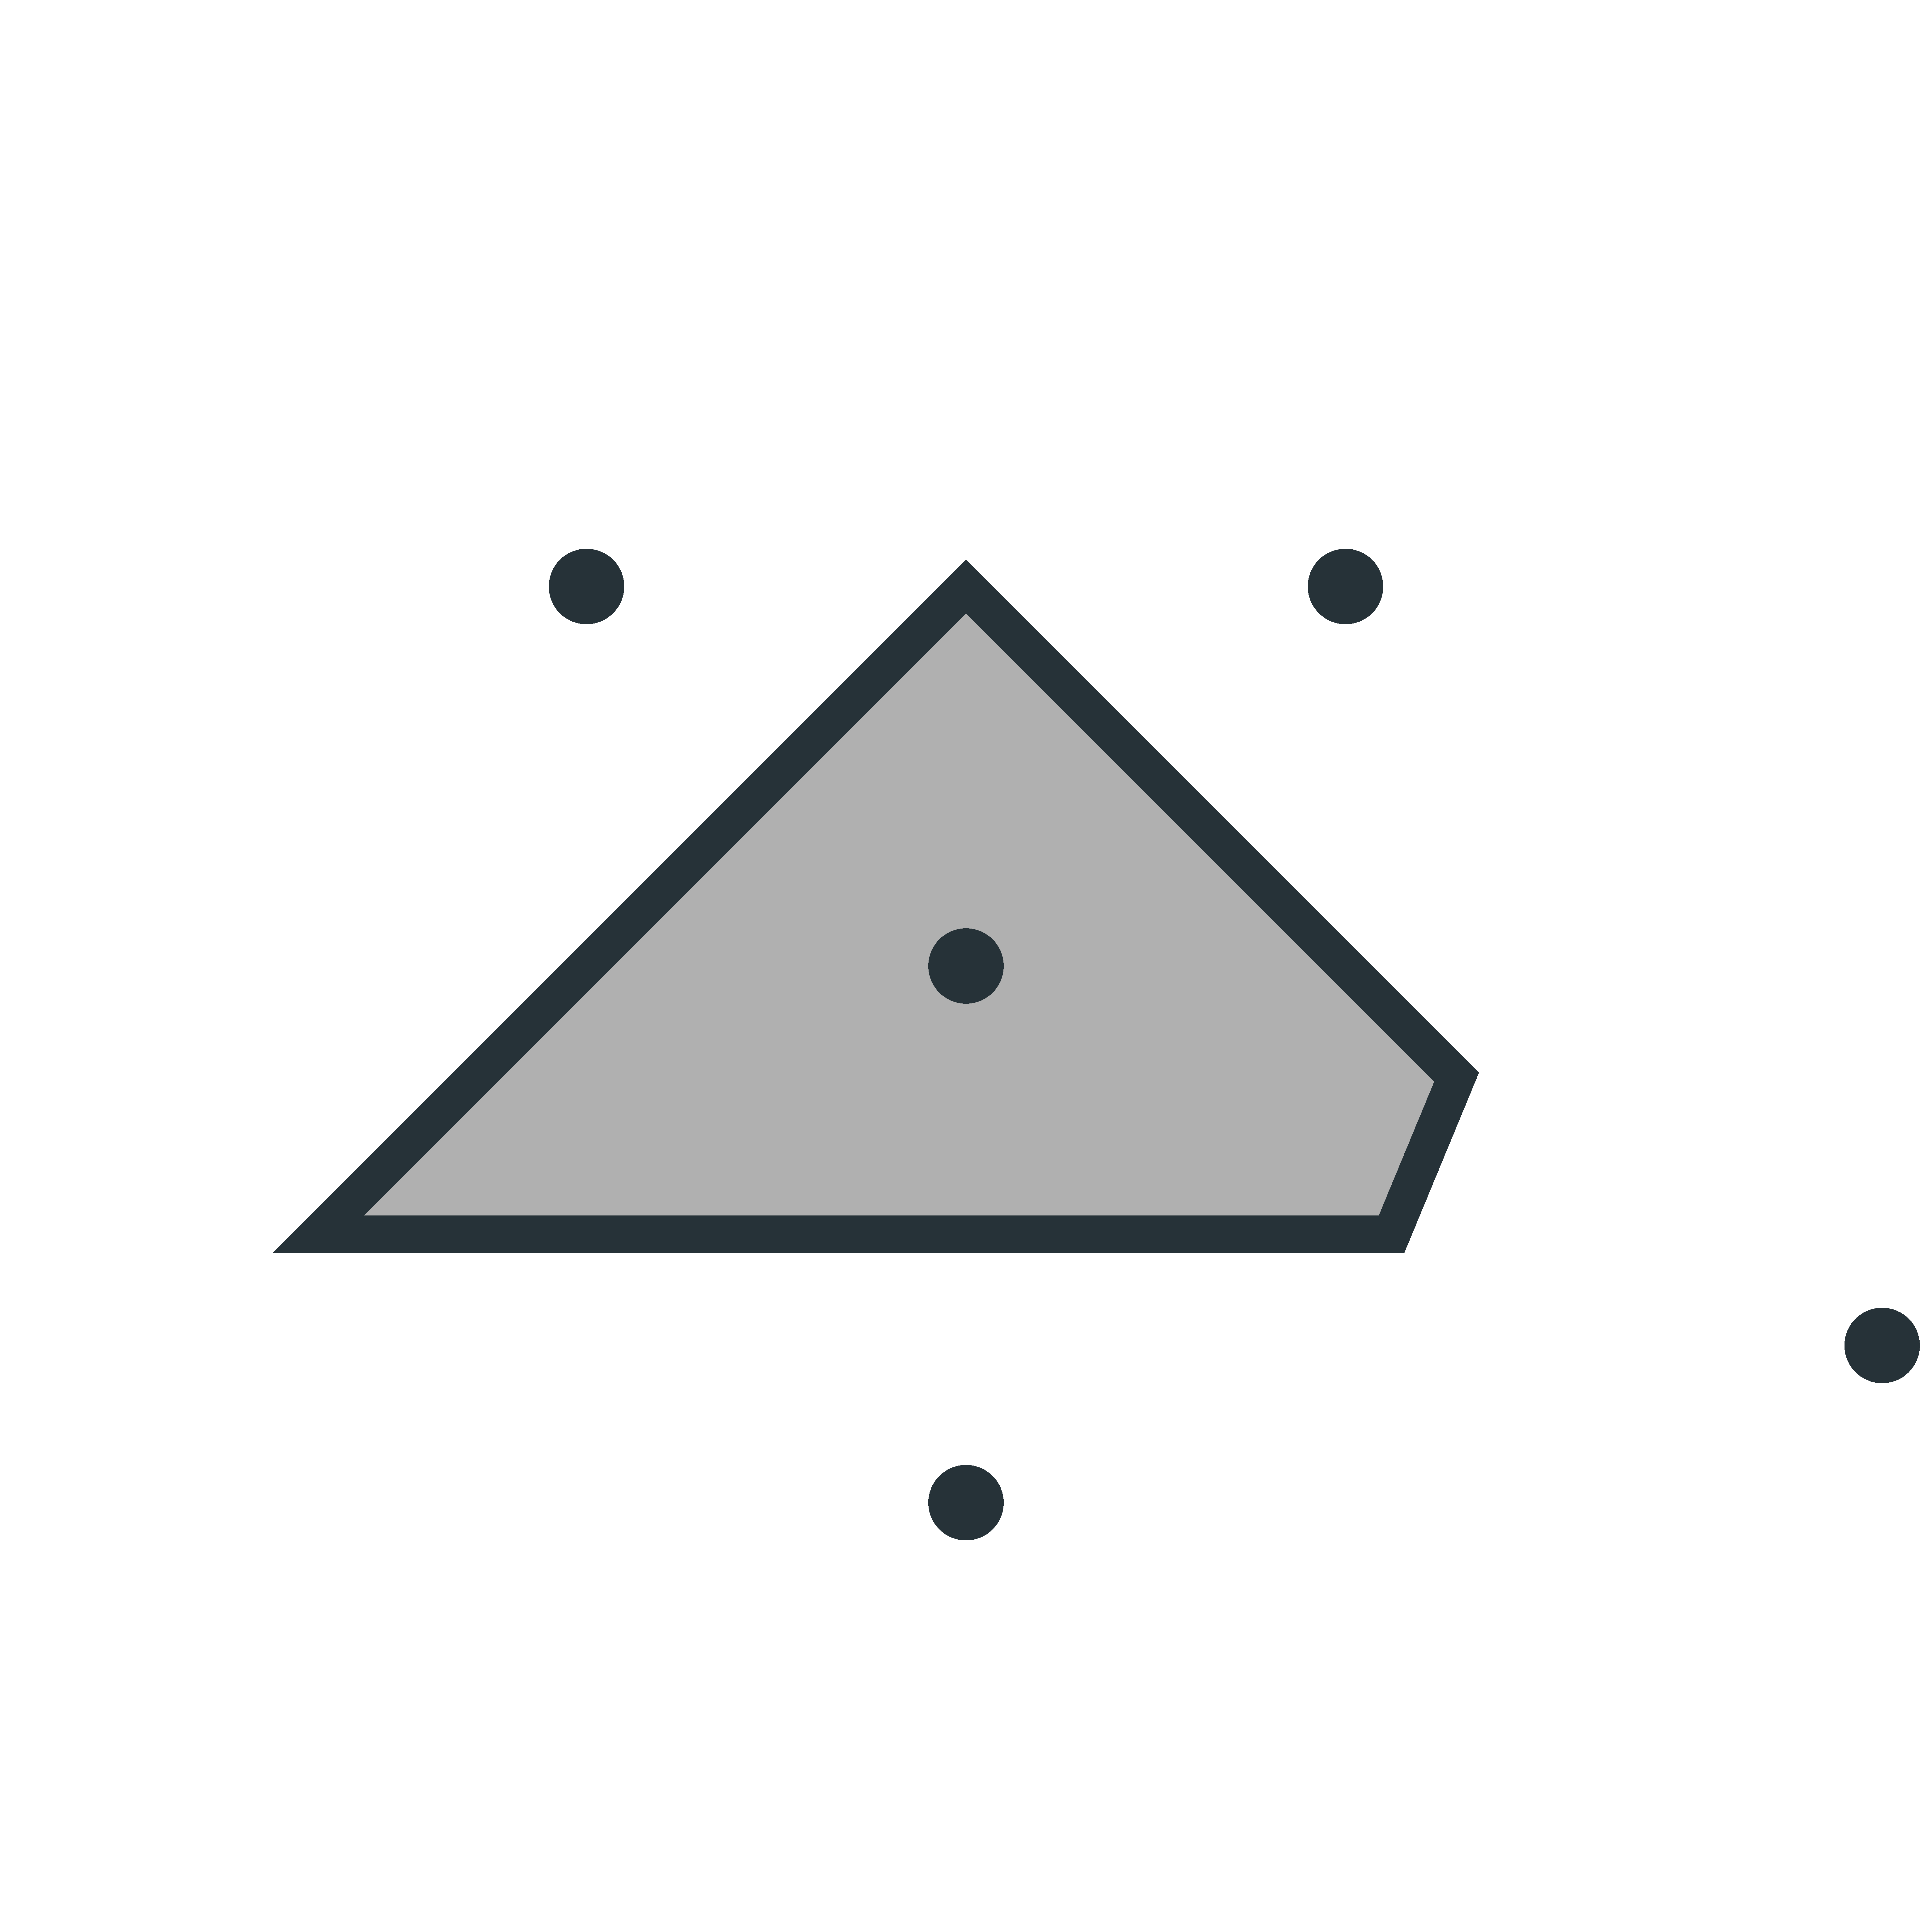
\includegraphics[width=0.11\textwidth]{img/results/tiles/octagon_100000_(1_0alpha_1)_020.pdf}
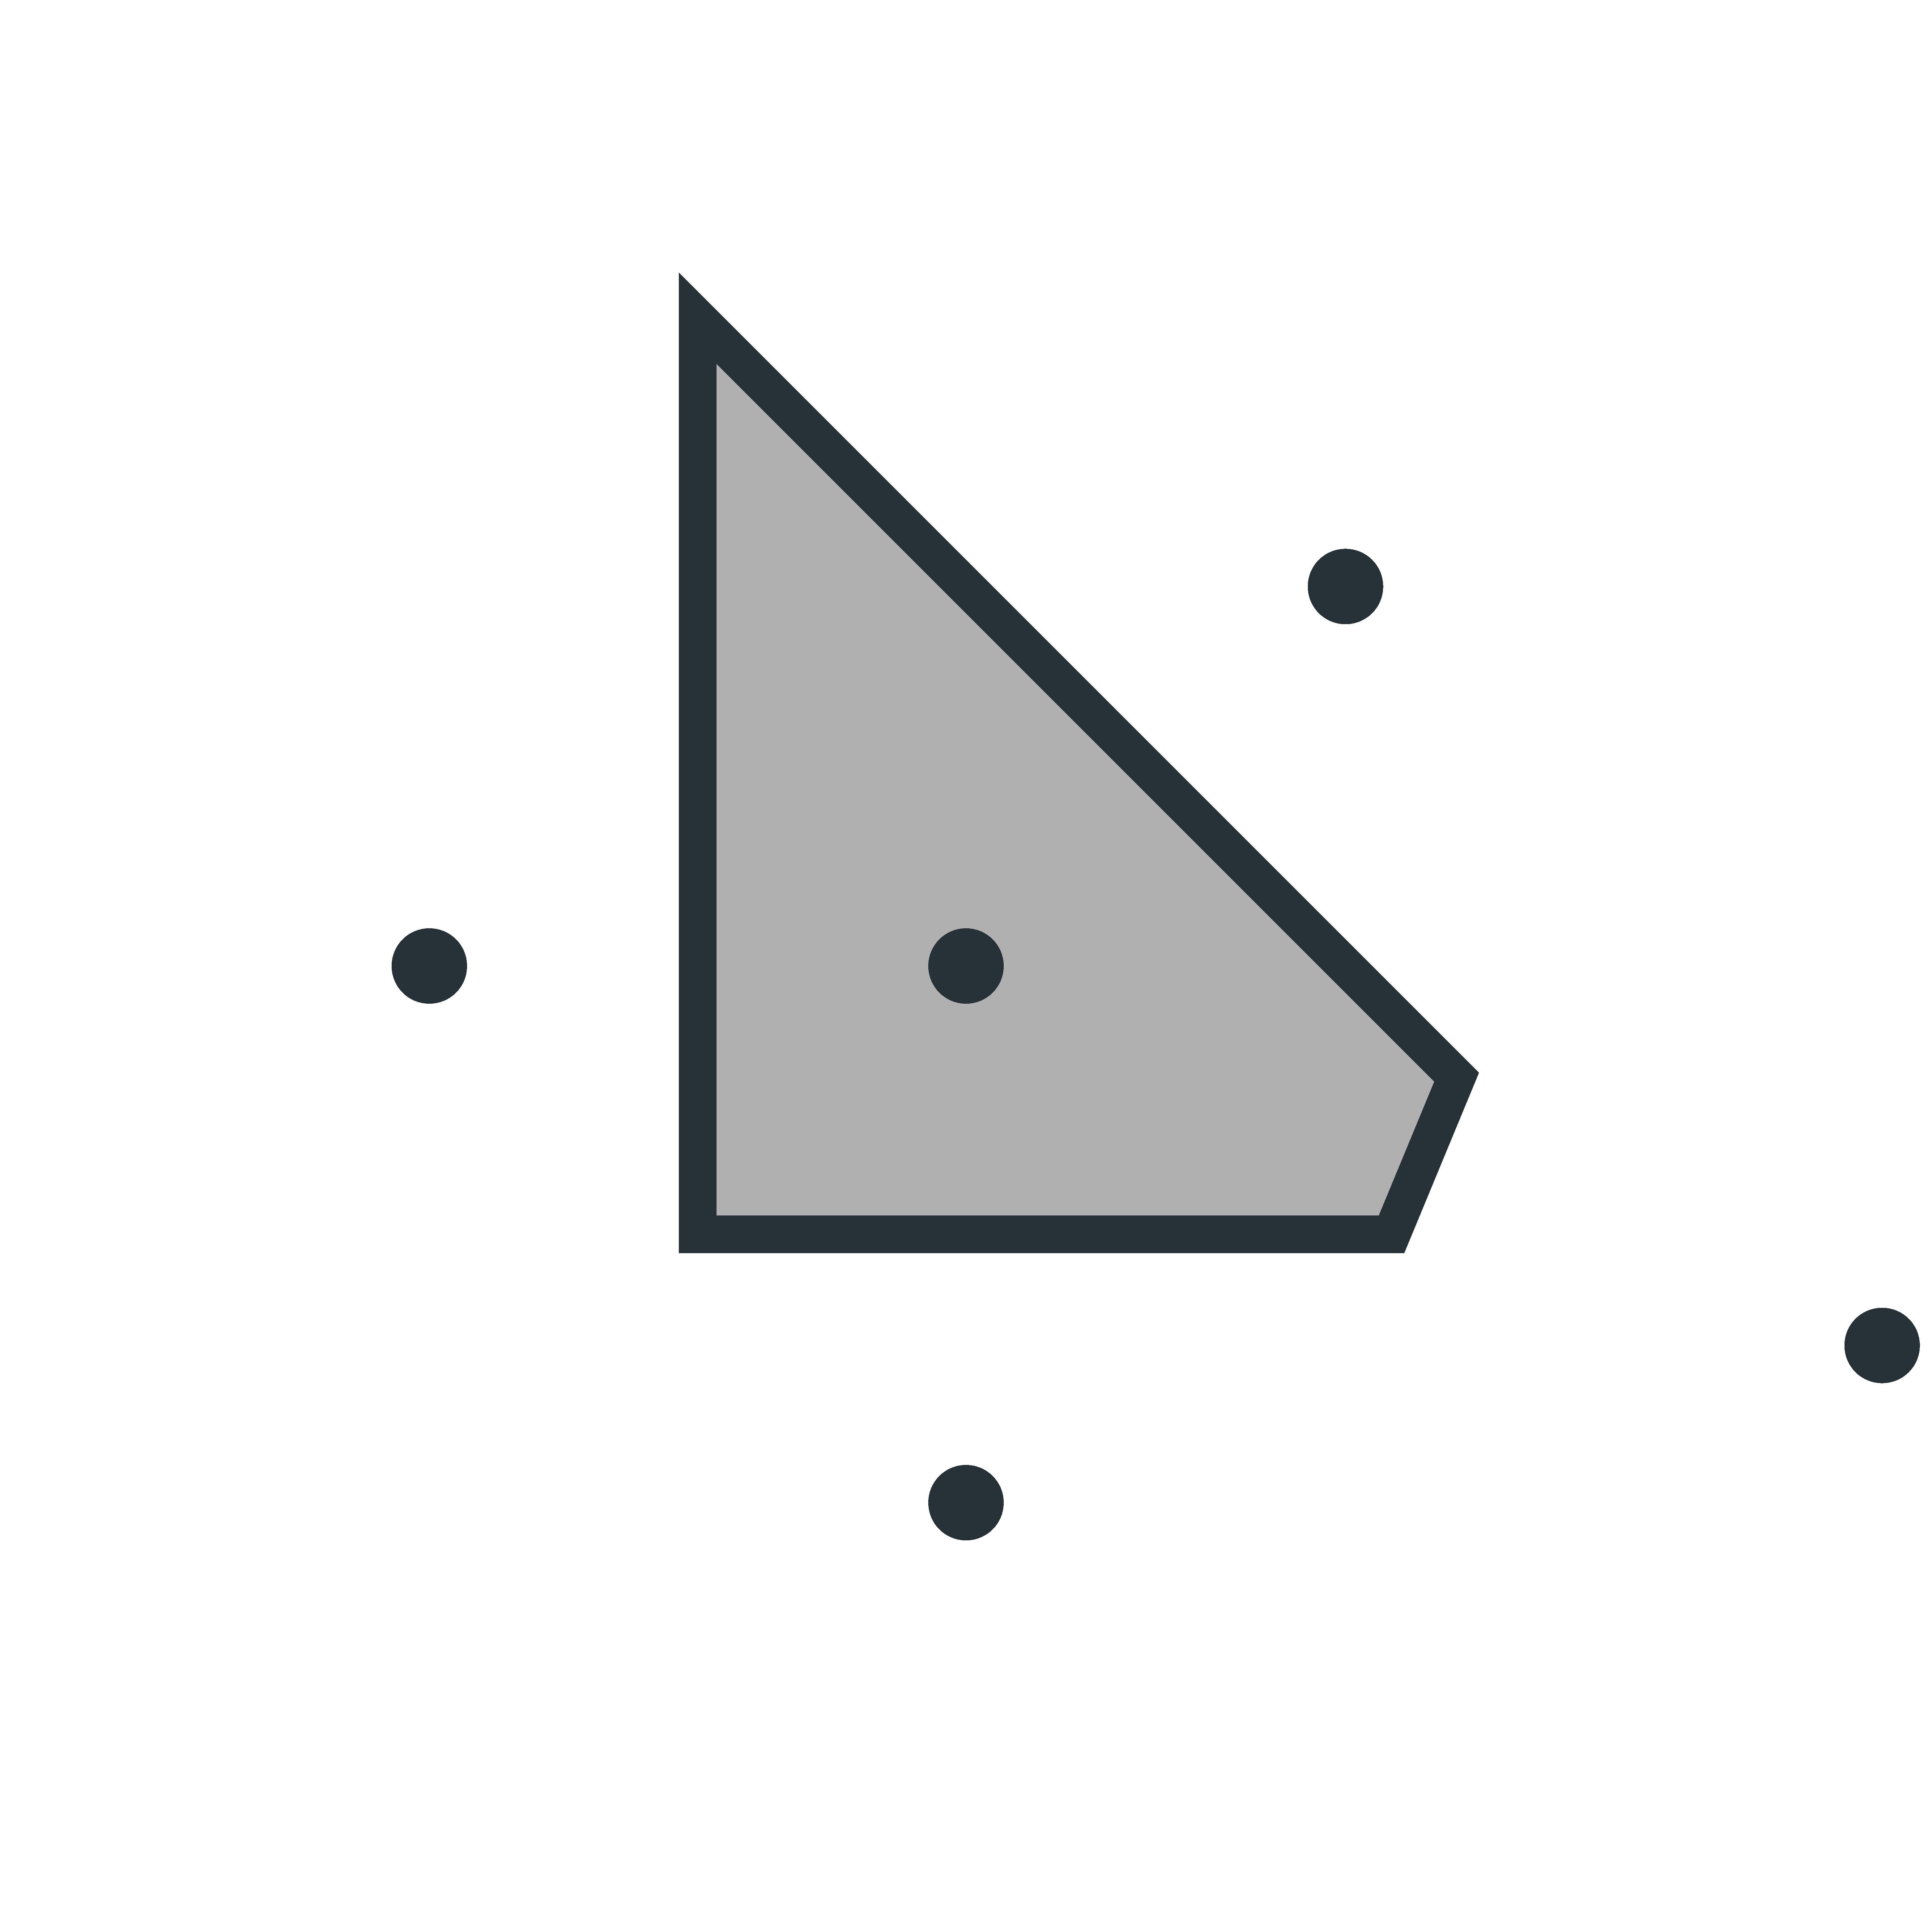
\includegraphics[width=0.11\textwidth]{img/results/tiles/octagon_100000_(1_0alpha_1)_021.pdf}
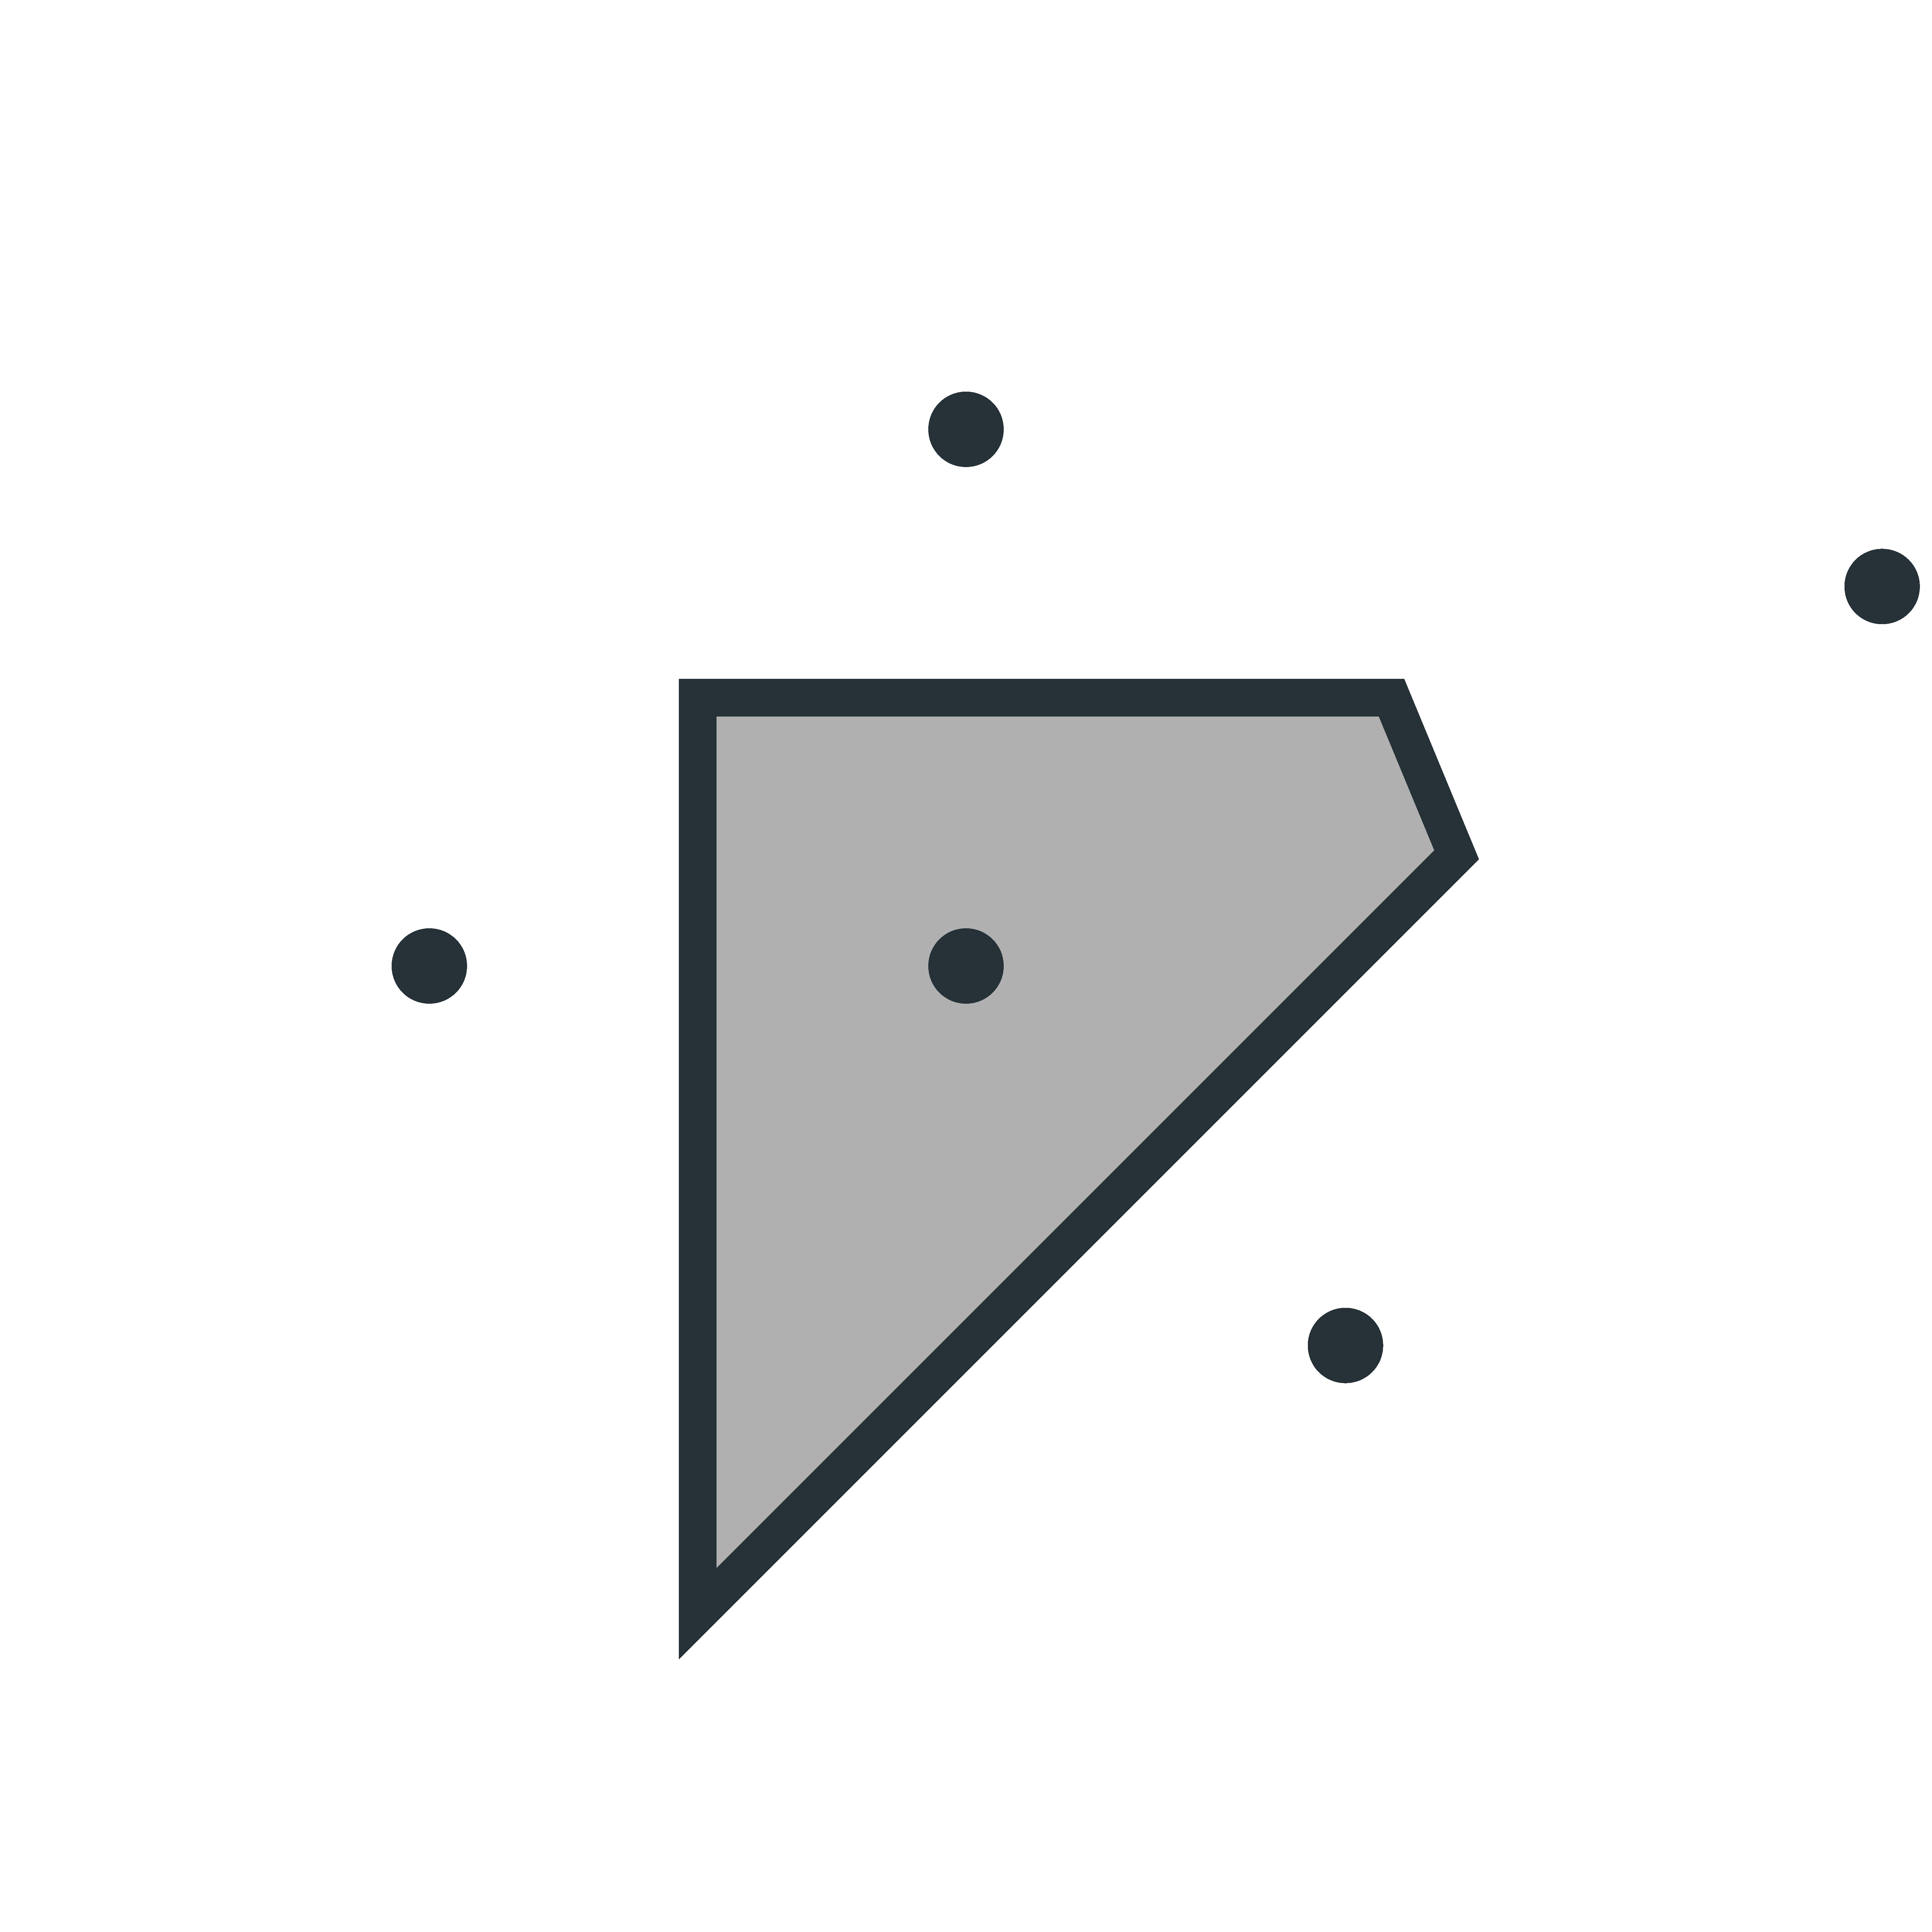
\includegraphics[width=0.11\textwidth]{img/results/tiles/octagon_100000_(1_0alpha_1)_022.pdf}
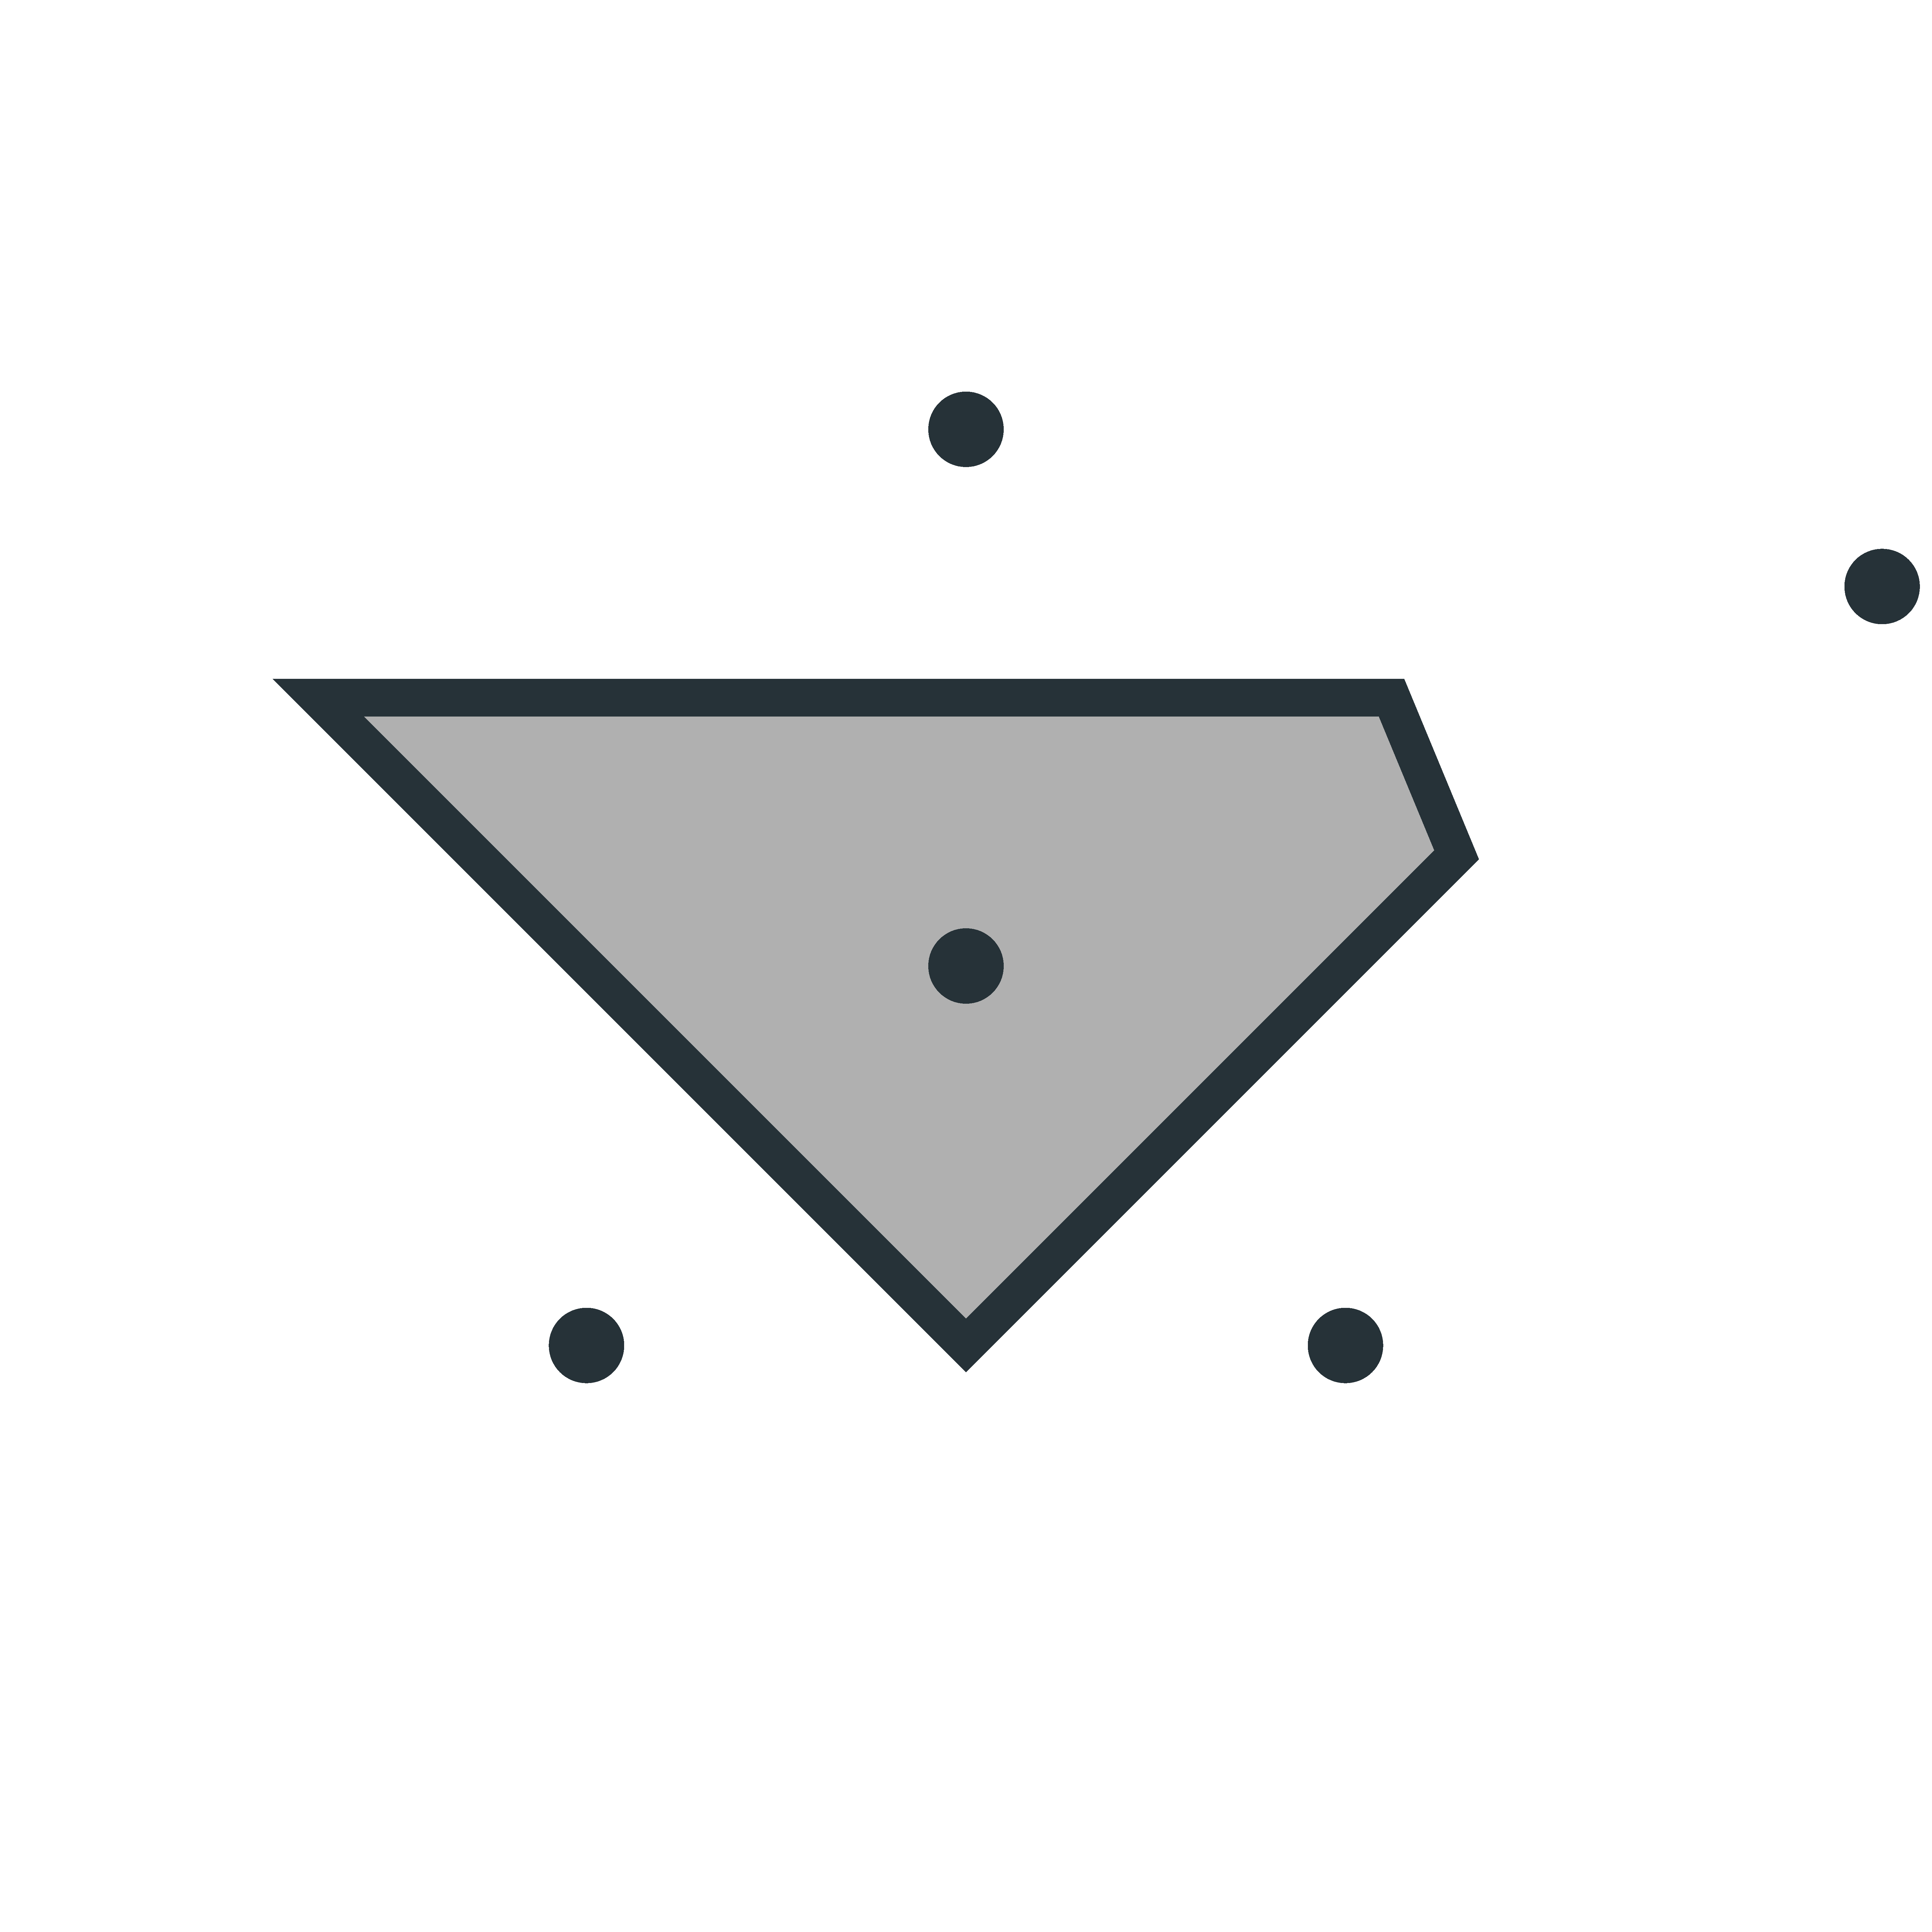
\includegraphics[width=0.11\textwidth]{img/results/tiles/octagon_100000_(1_0alpha_1)_023.pdf}
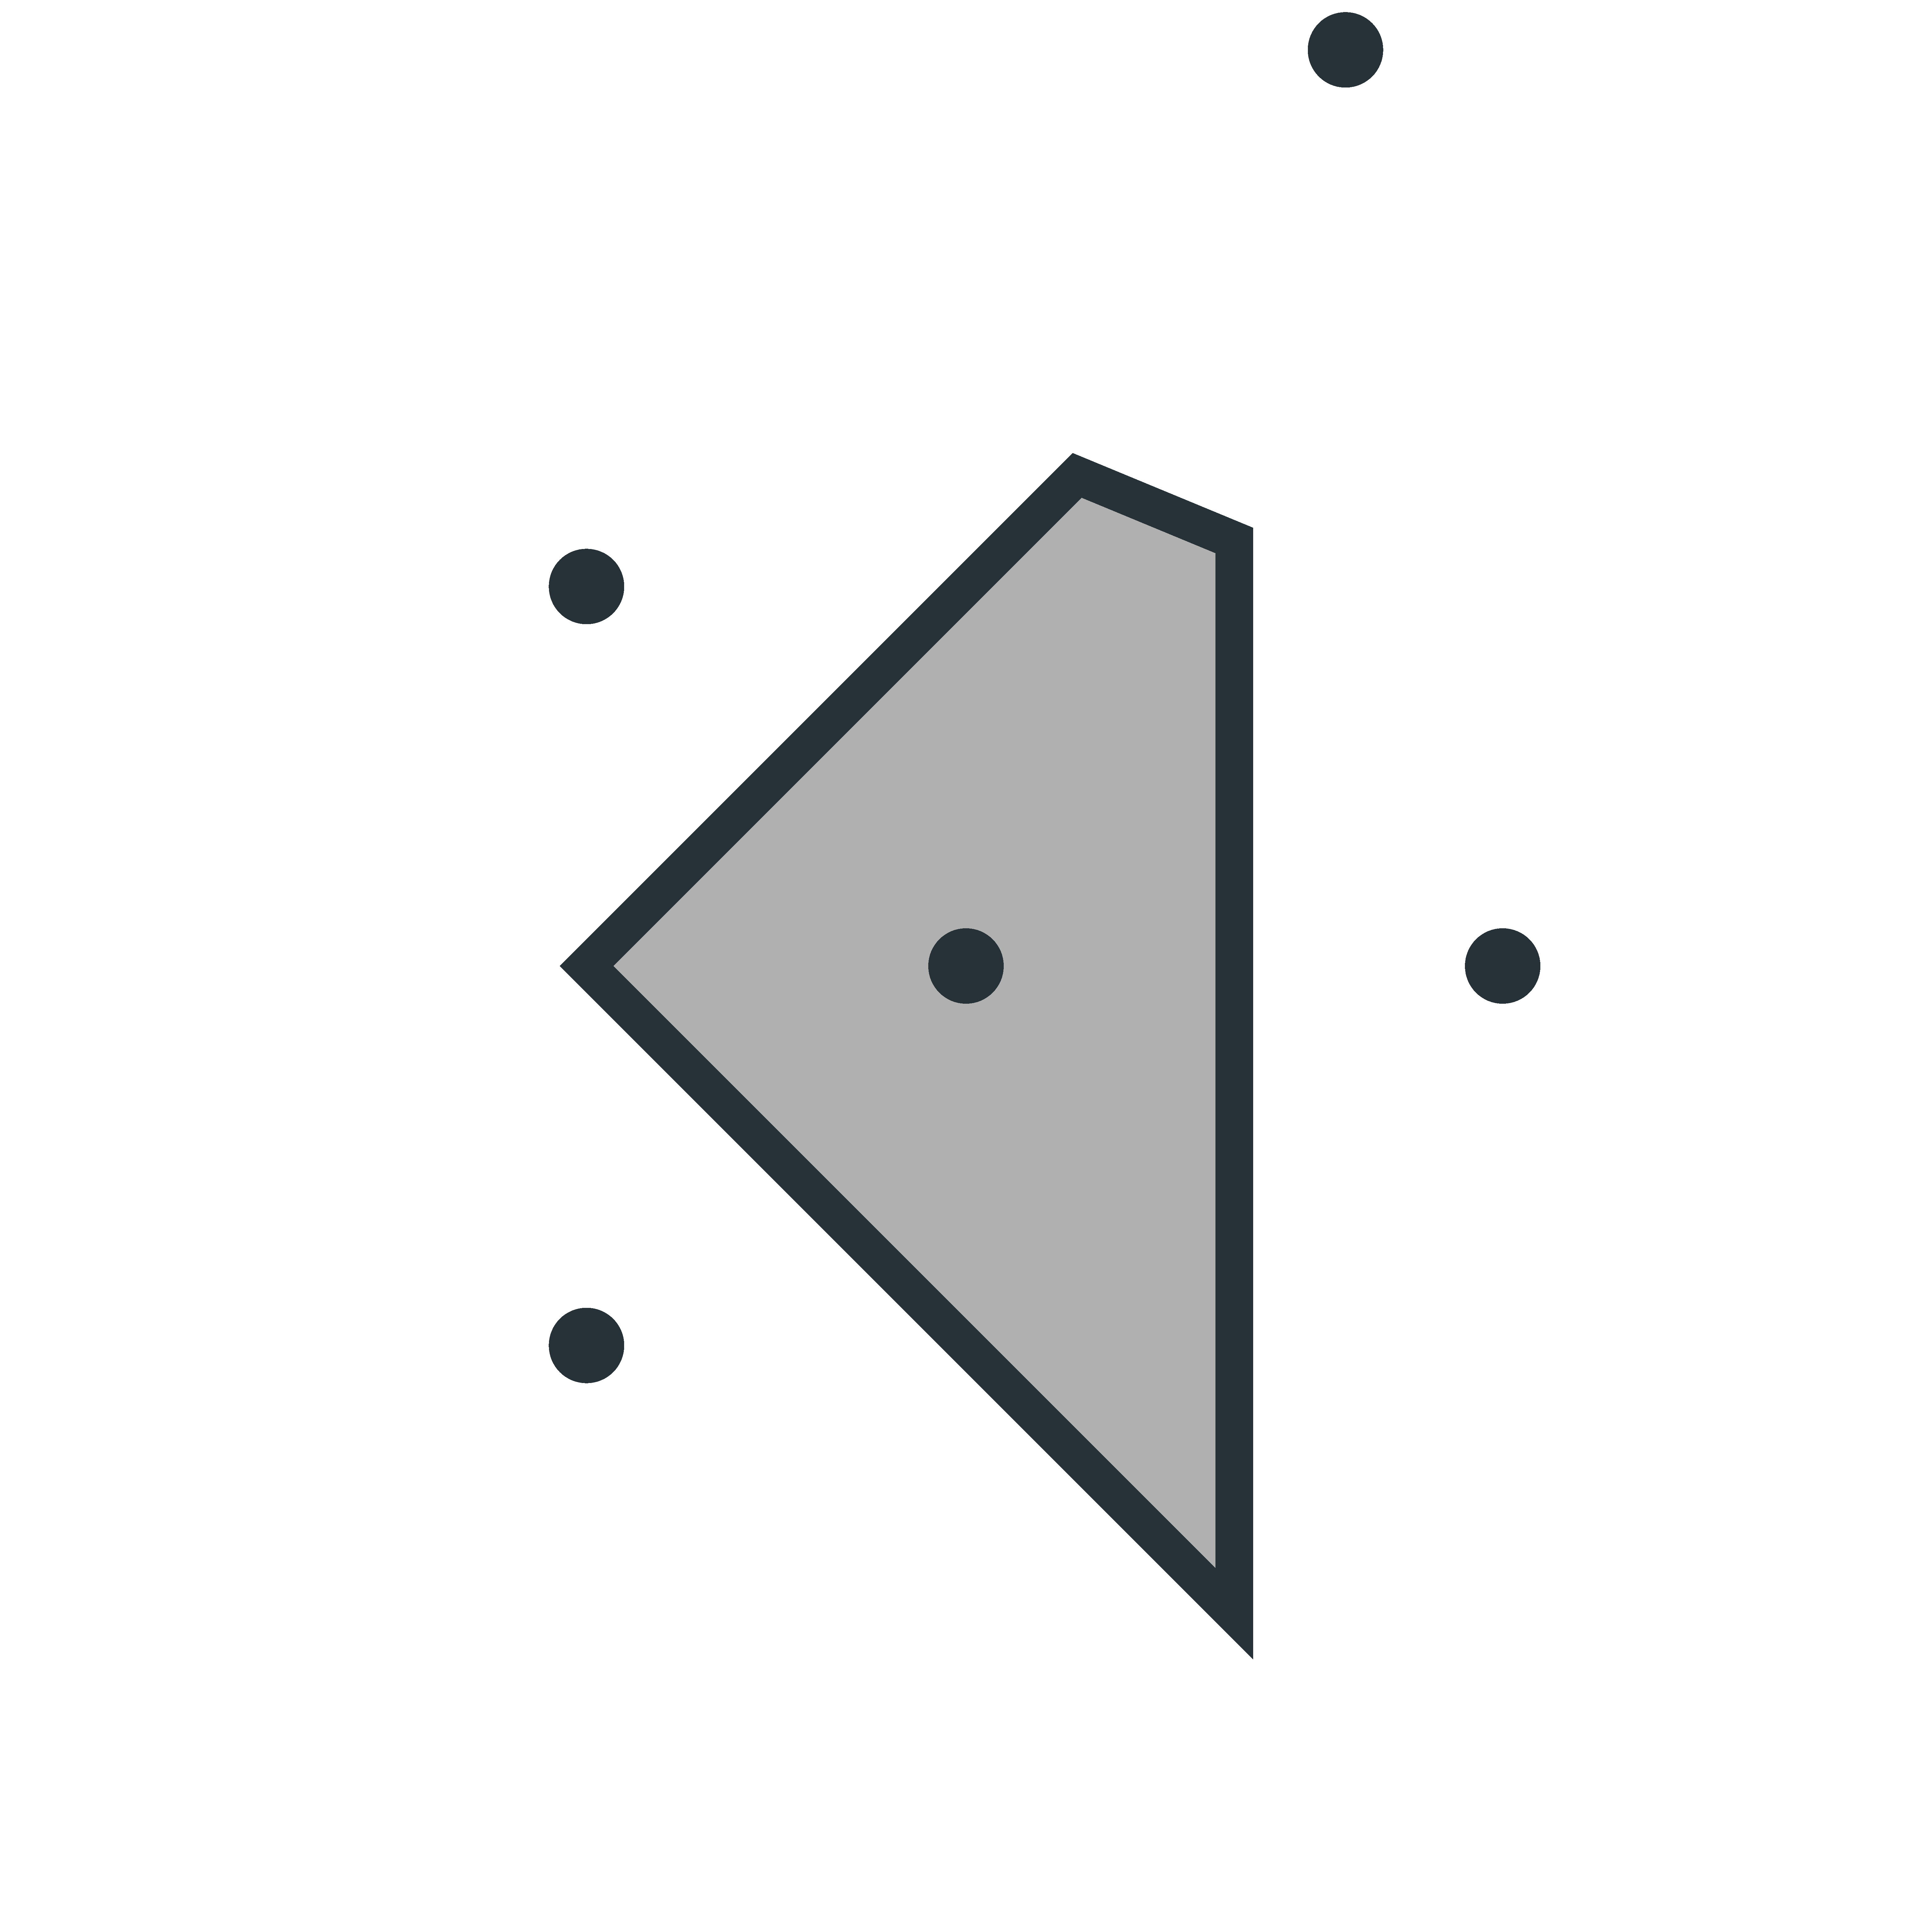
\includegraphics[width=0.11\textwidth]{img/results/tiles/octagon_100000_(1_0alpha_1)_024.pdf}
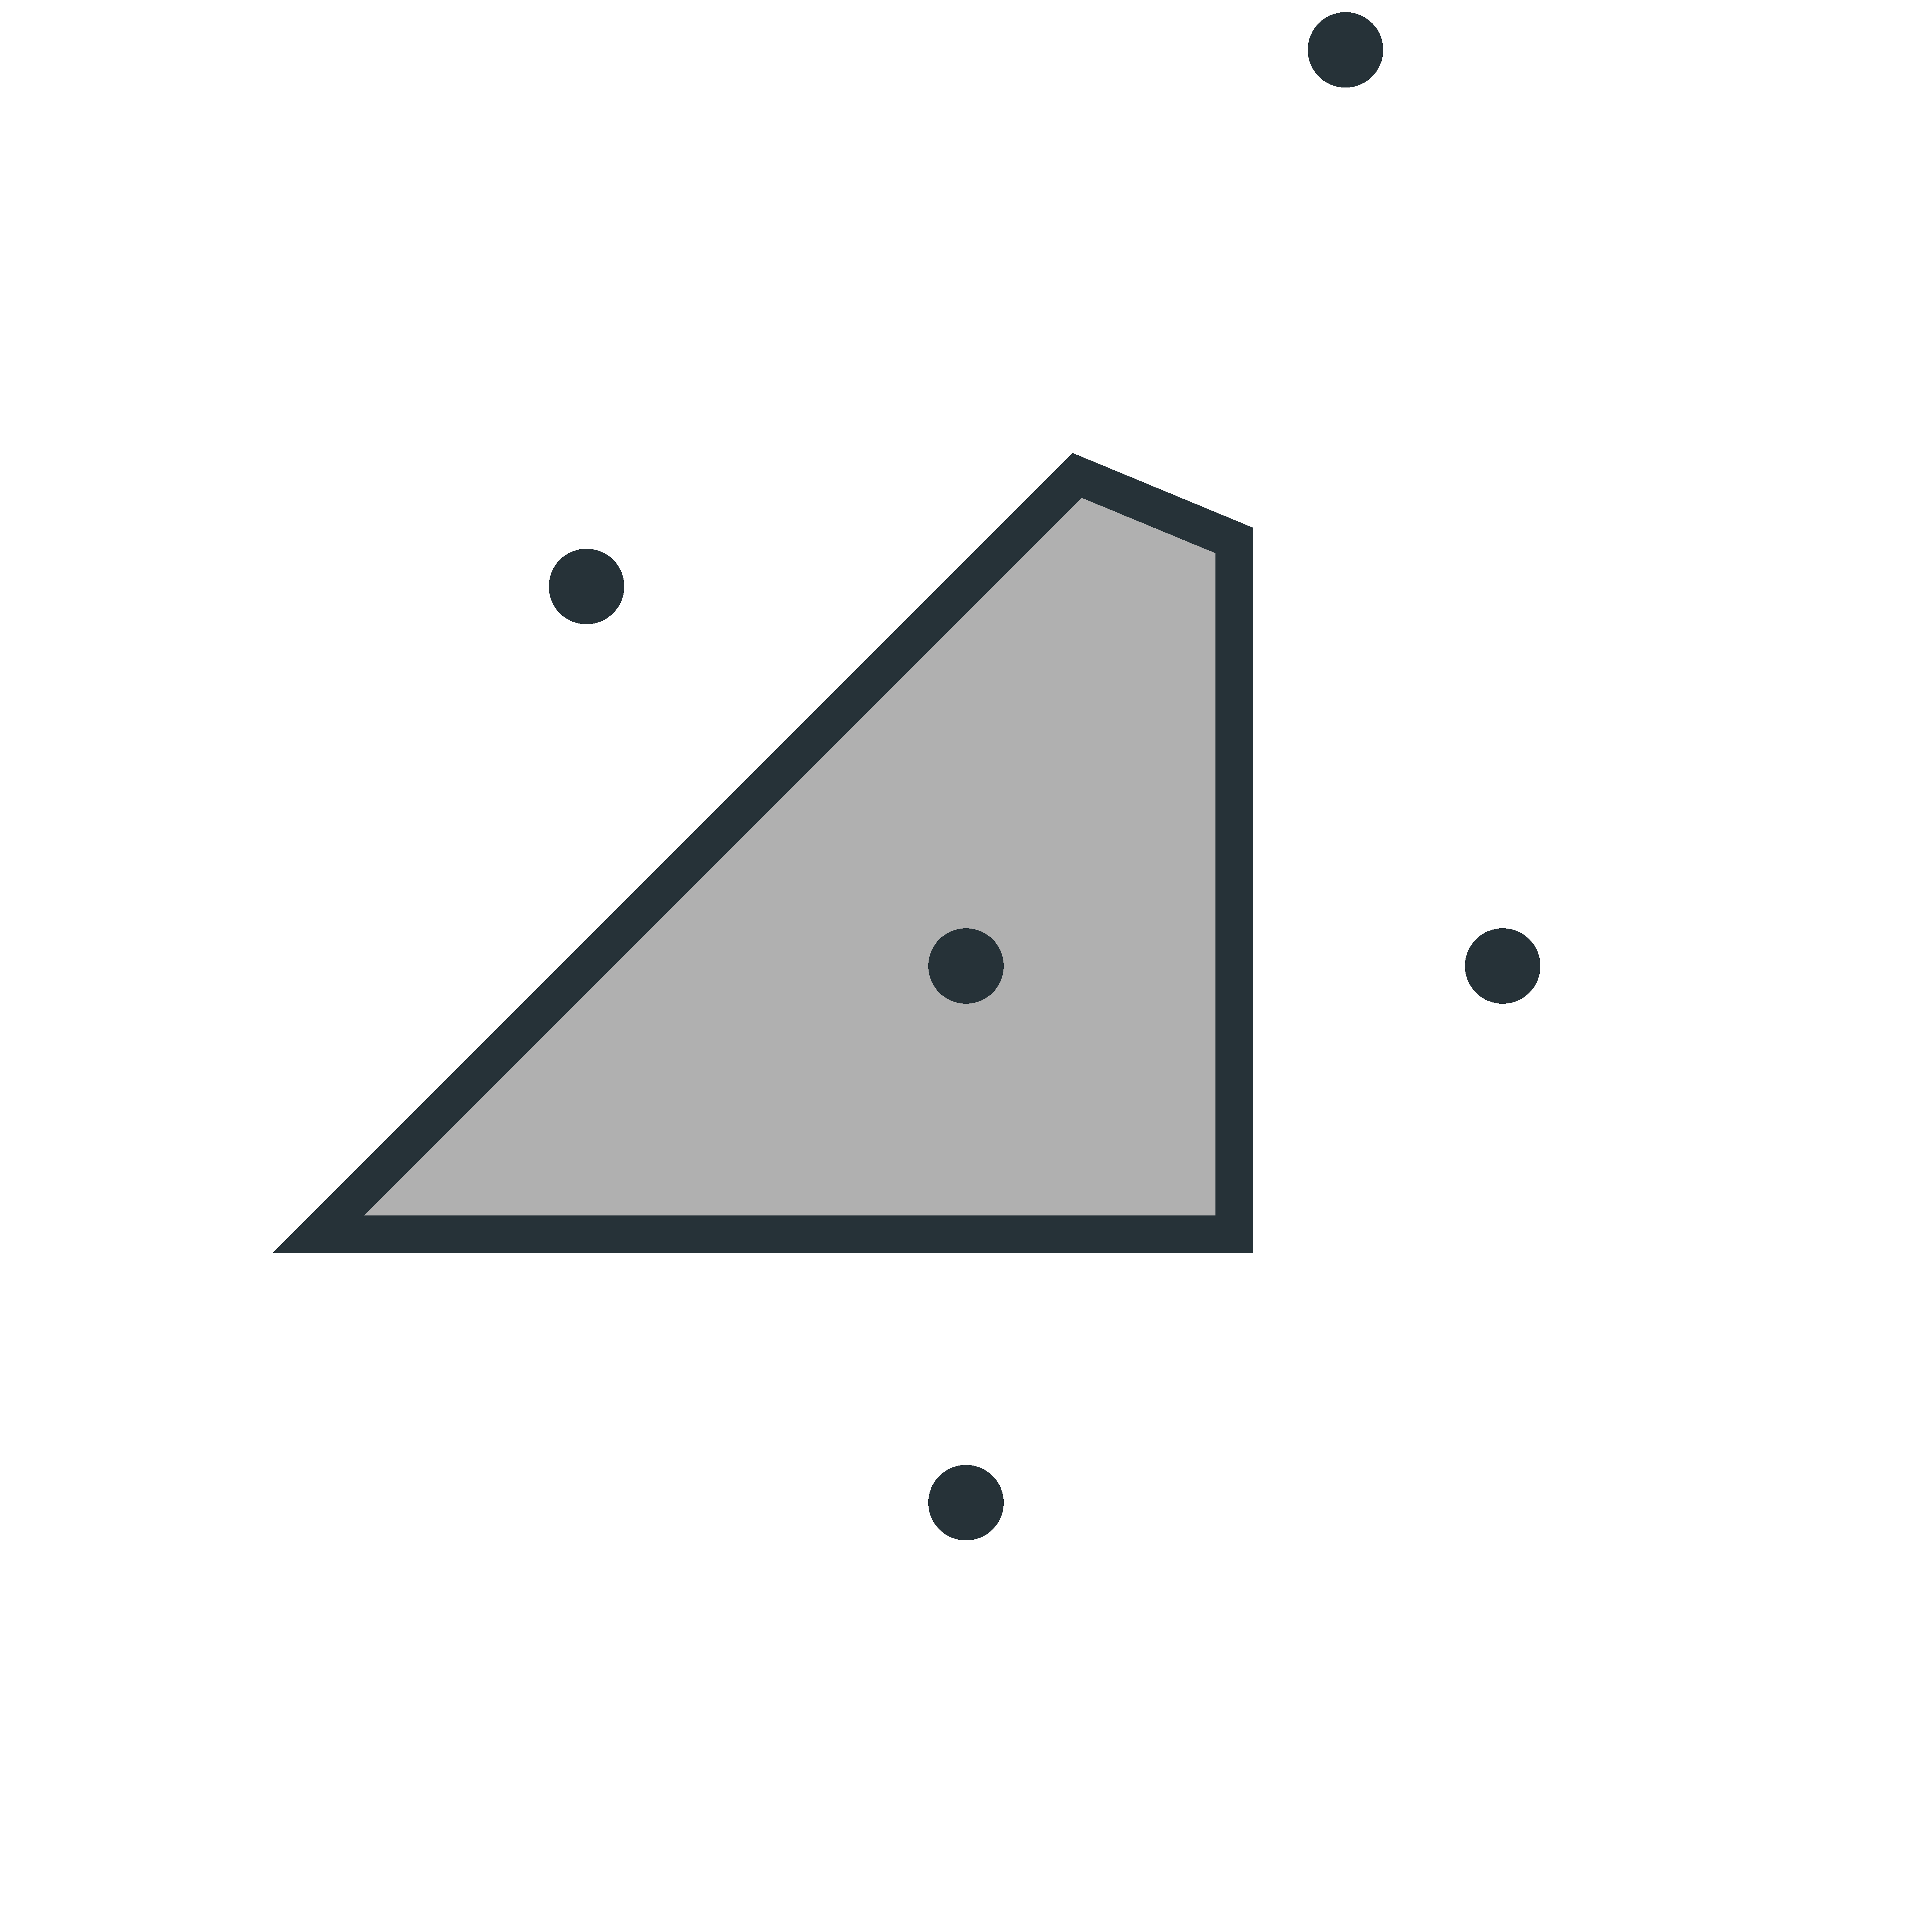
\includegraphics[width=0.11\textwidth]{img/results/tiles/octagon_100000_(1_0alpha_1)_025.pdf}
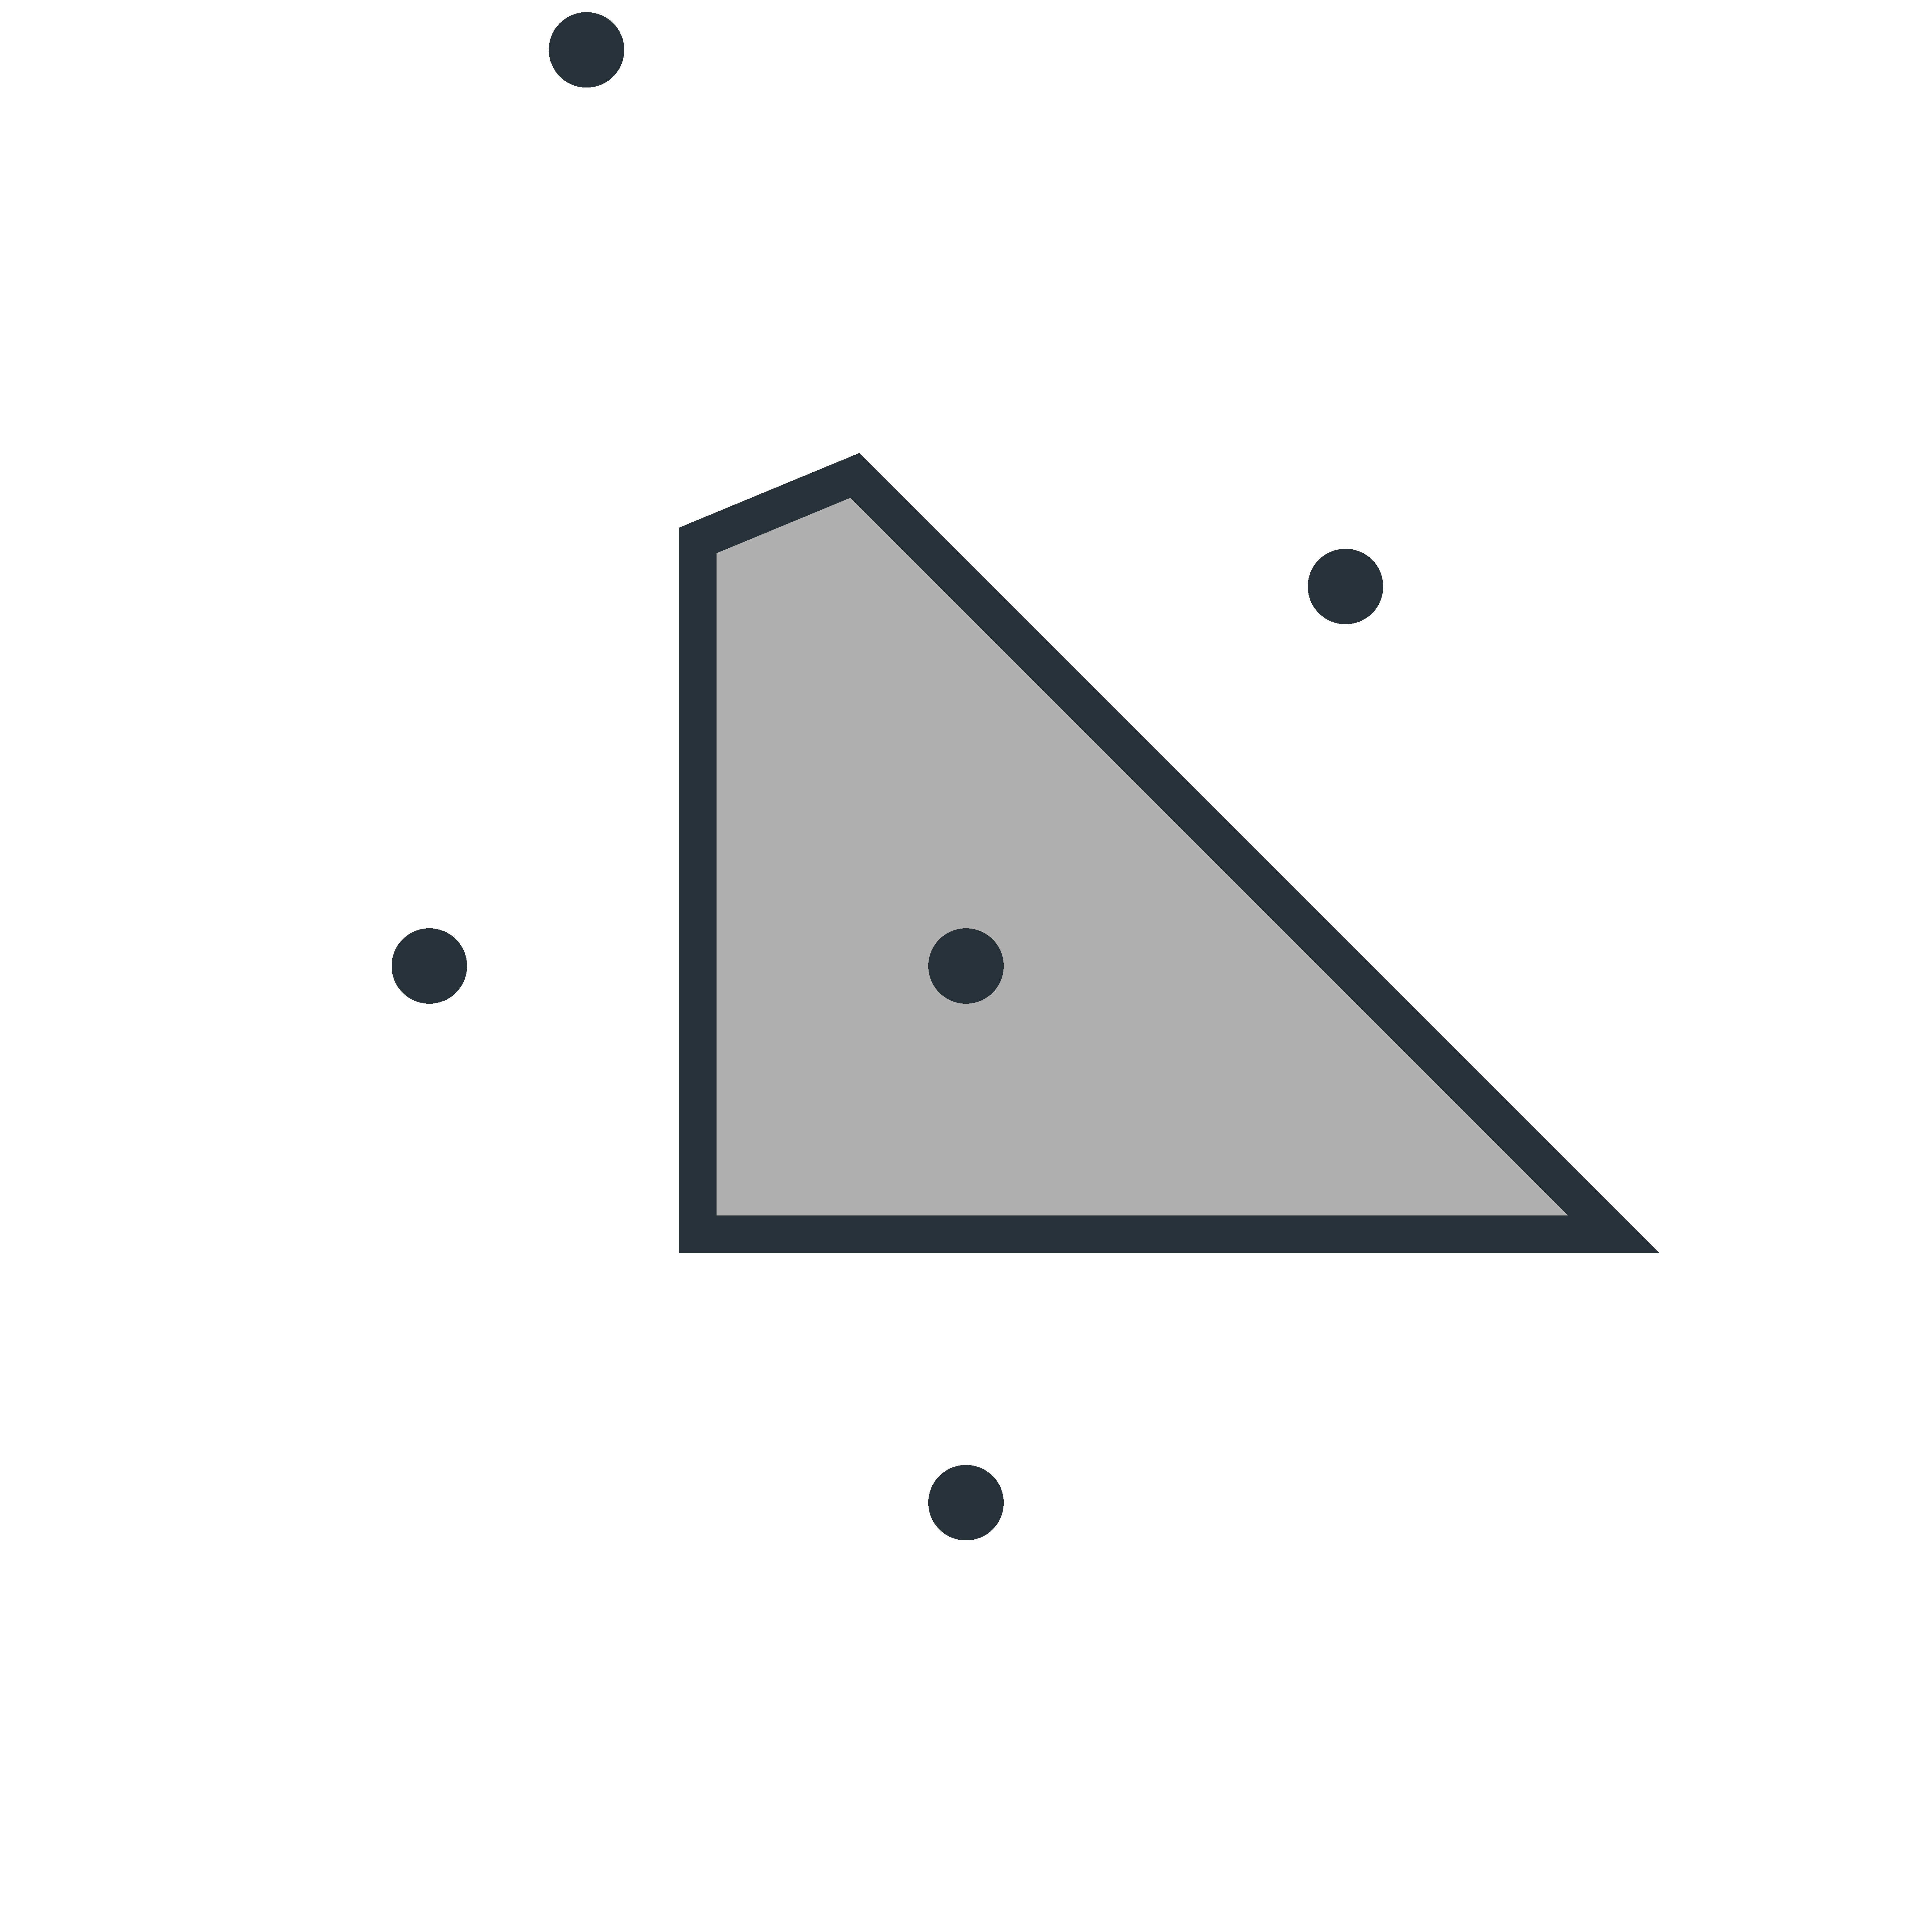
\includegraphics[width=0.11\textwidth]{img/results/tiles/octagon_100000_(1_0alpha_1)_026.pdf}
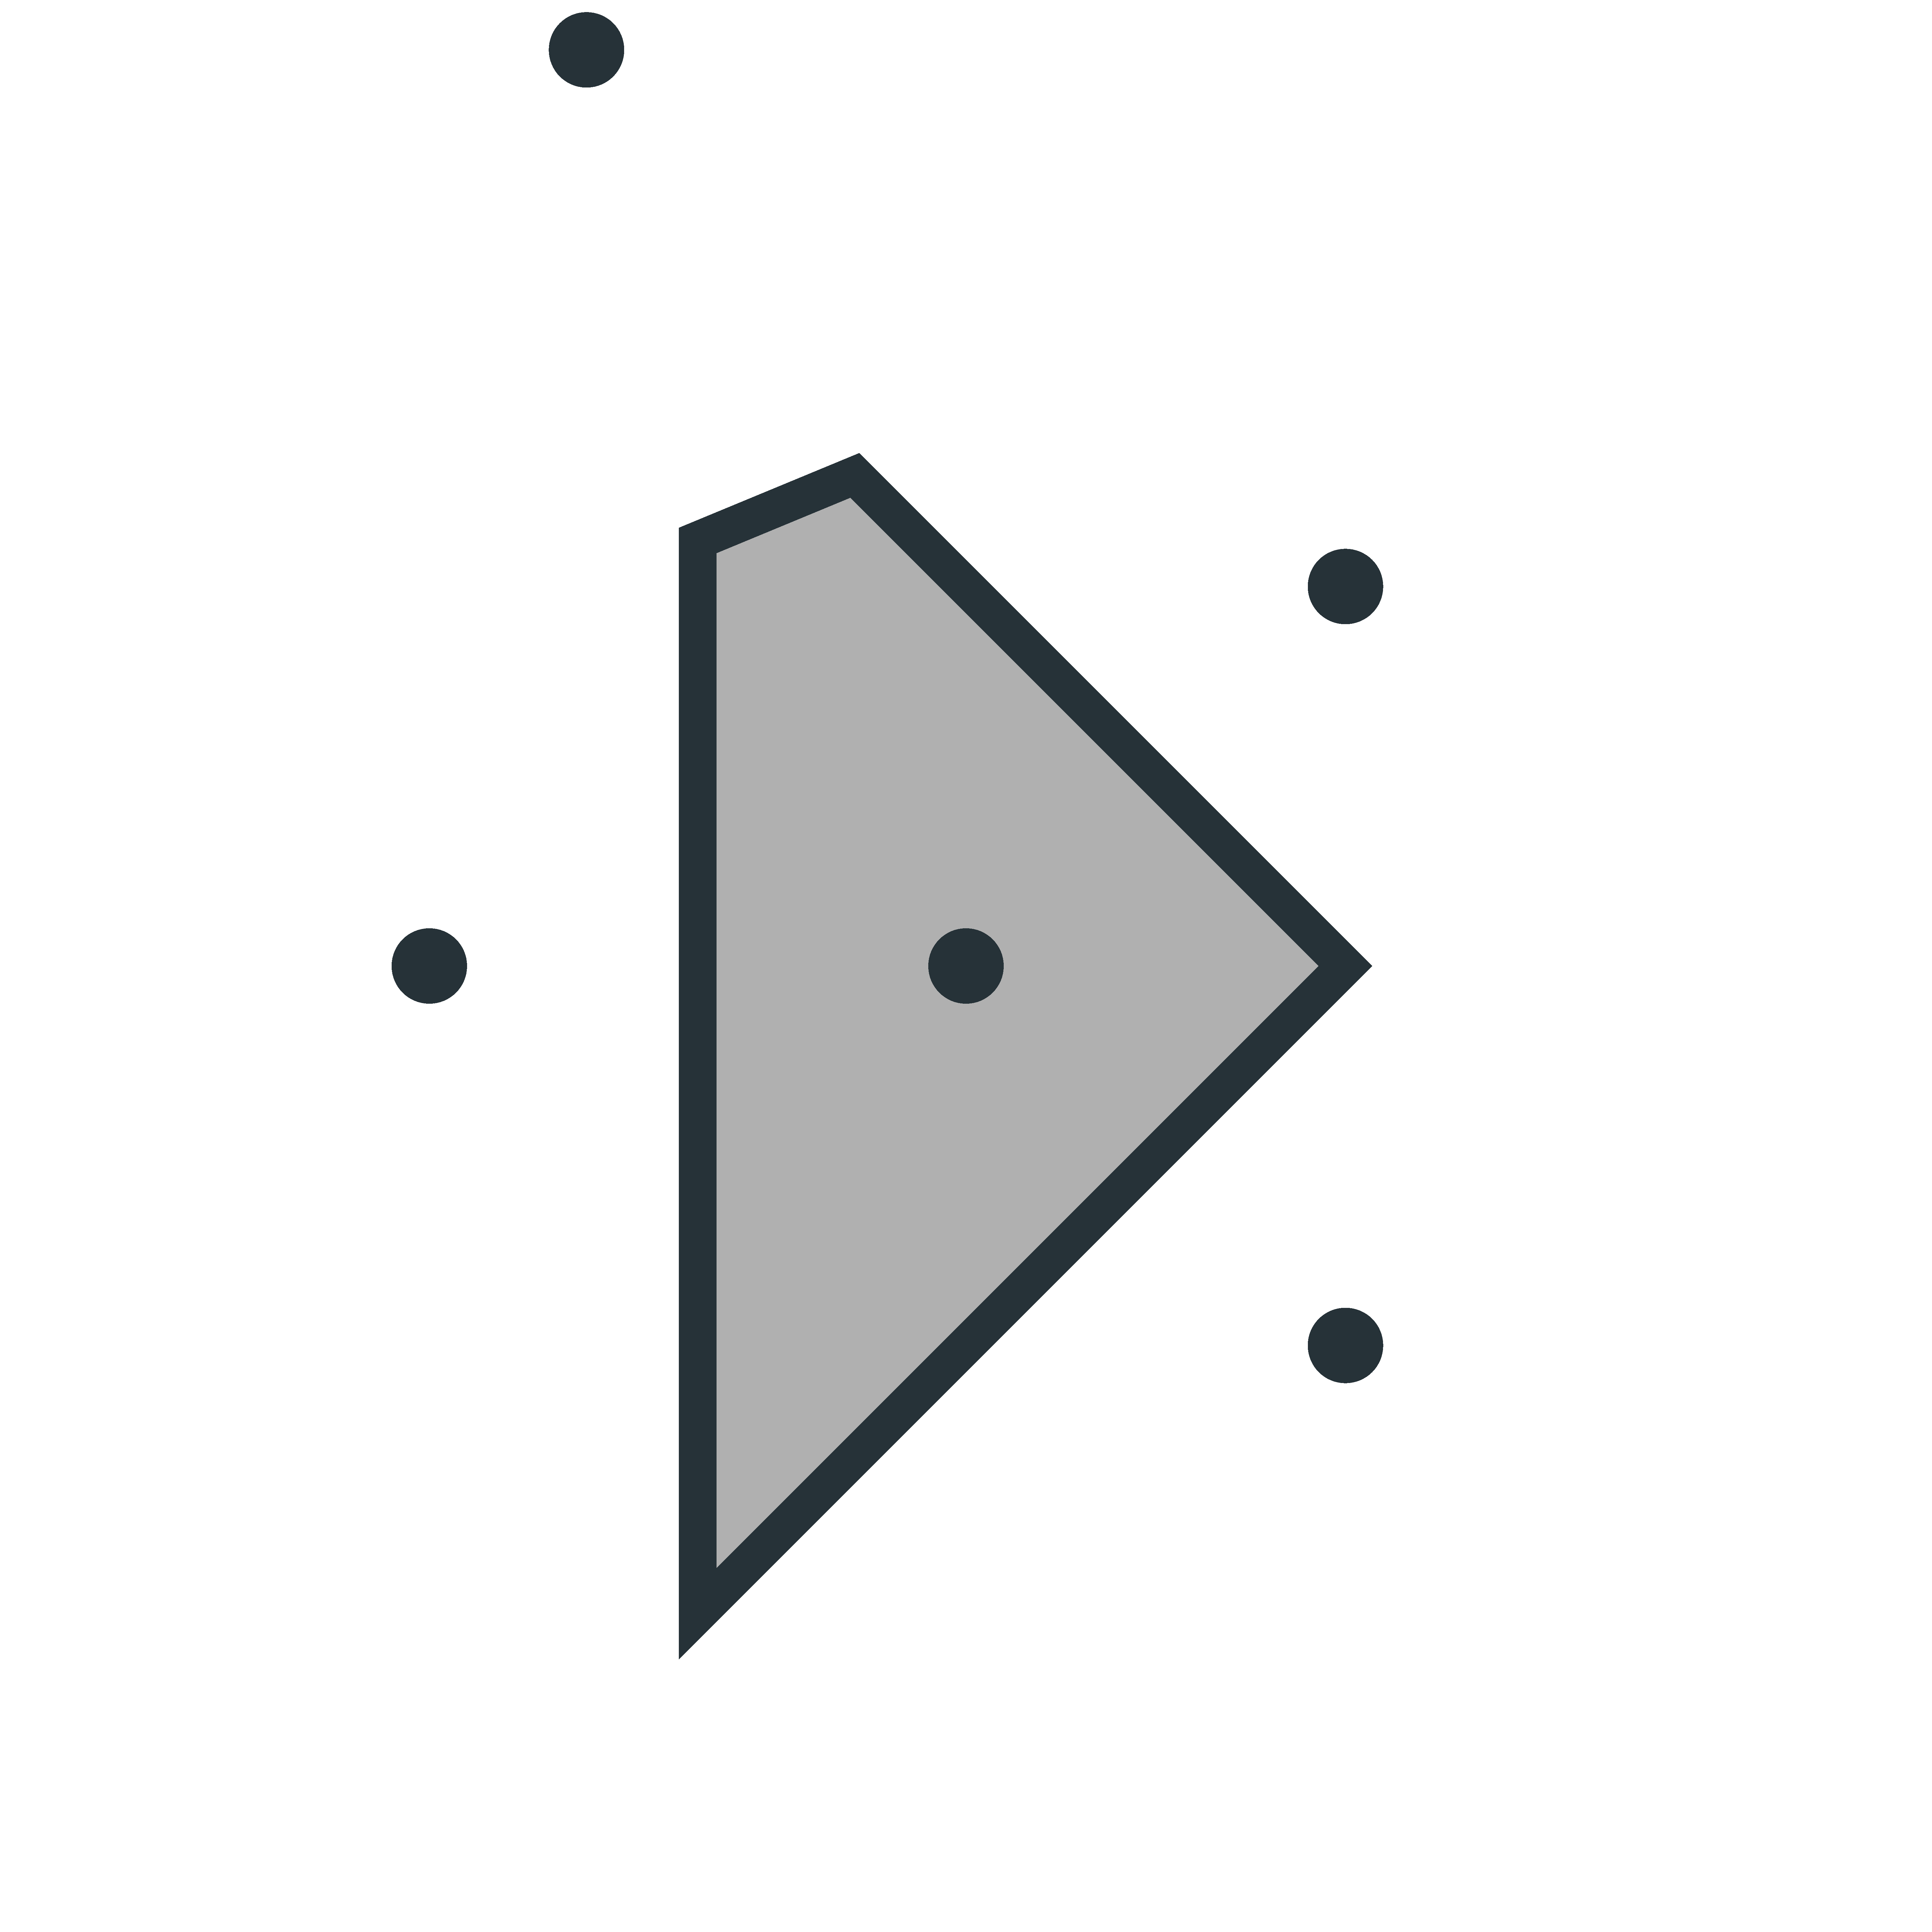
\includegraphics[width=0.11\textwidth]{img/results/tiles/octagon_100000_(1_0alpha_1)_027.pdf}
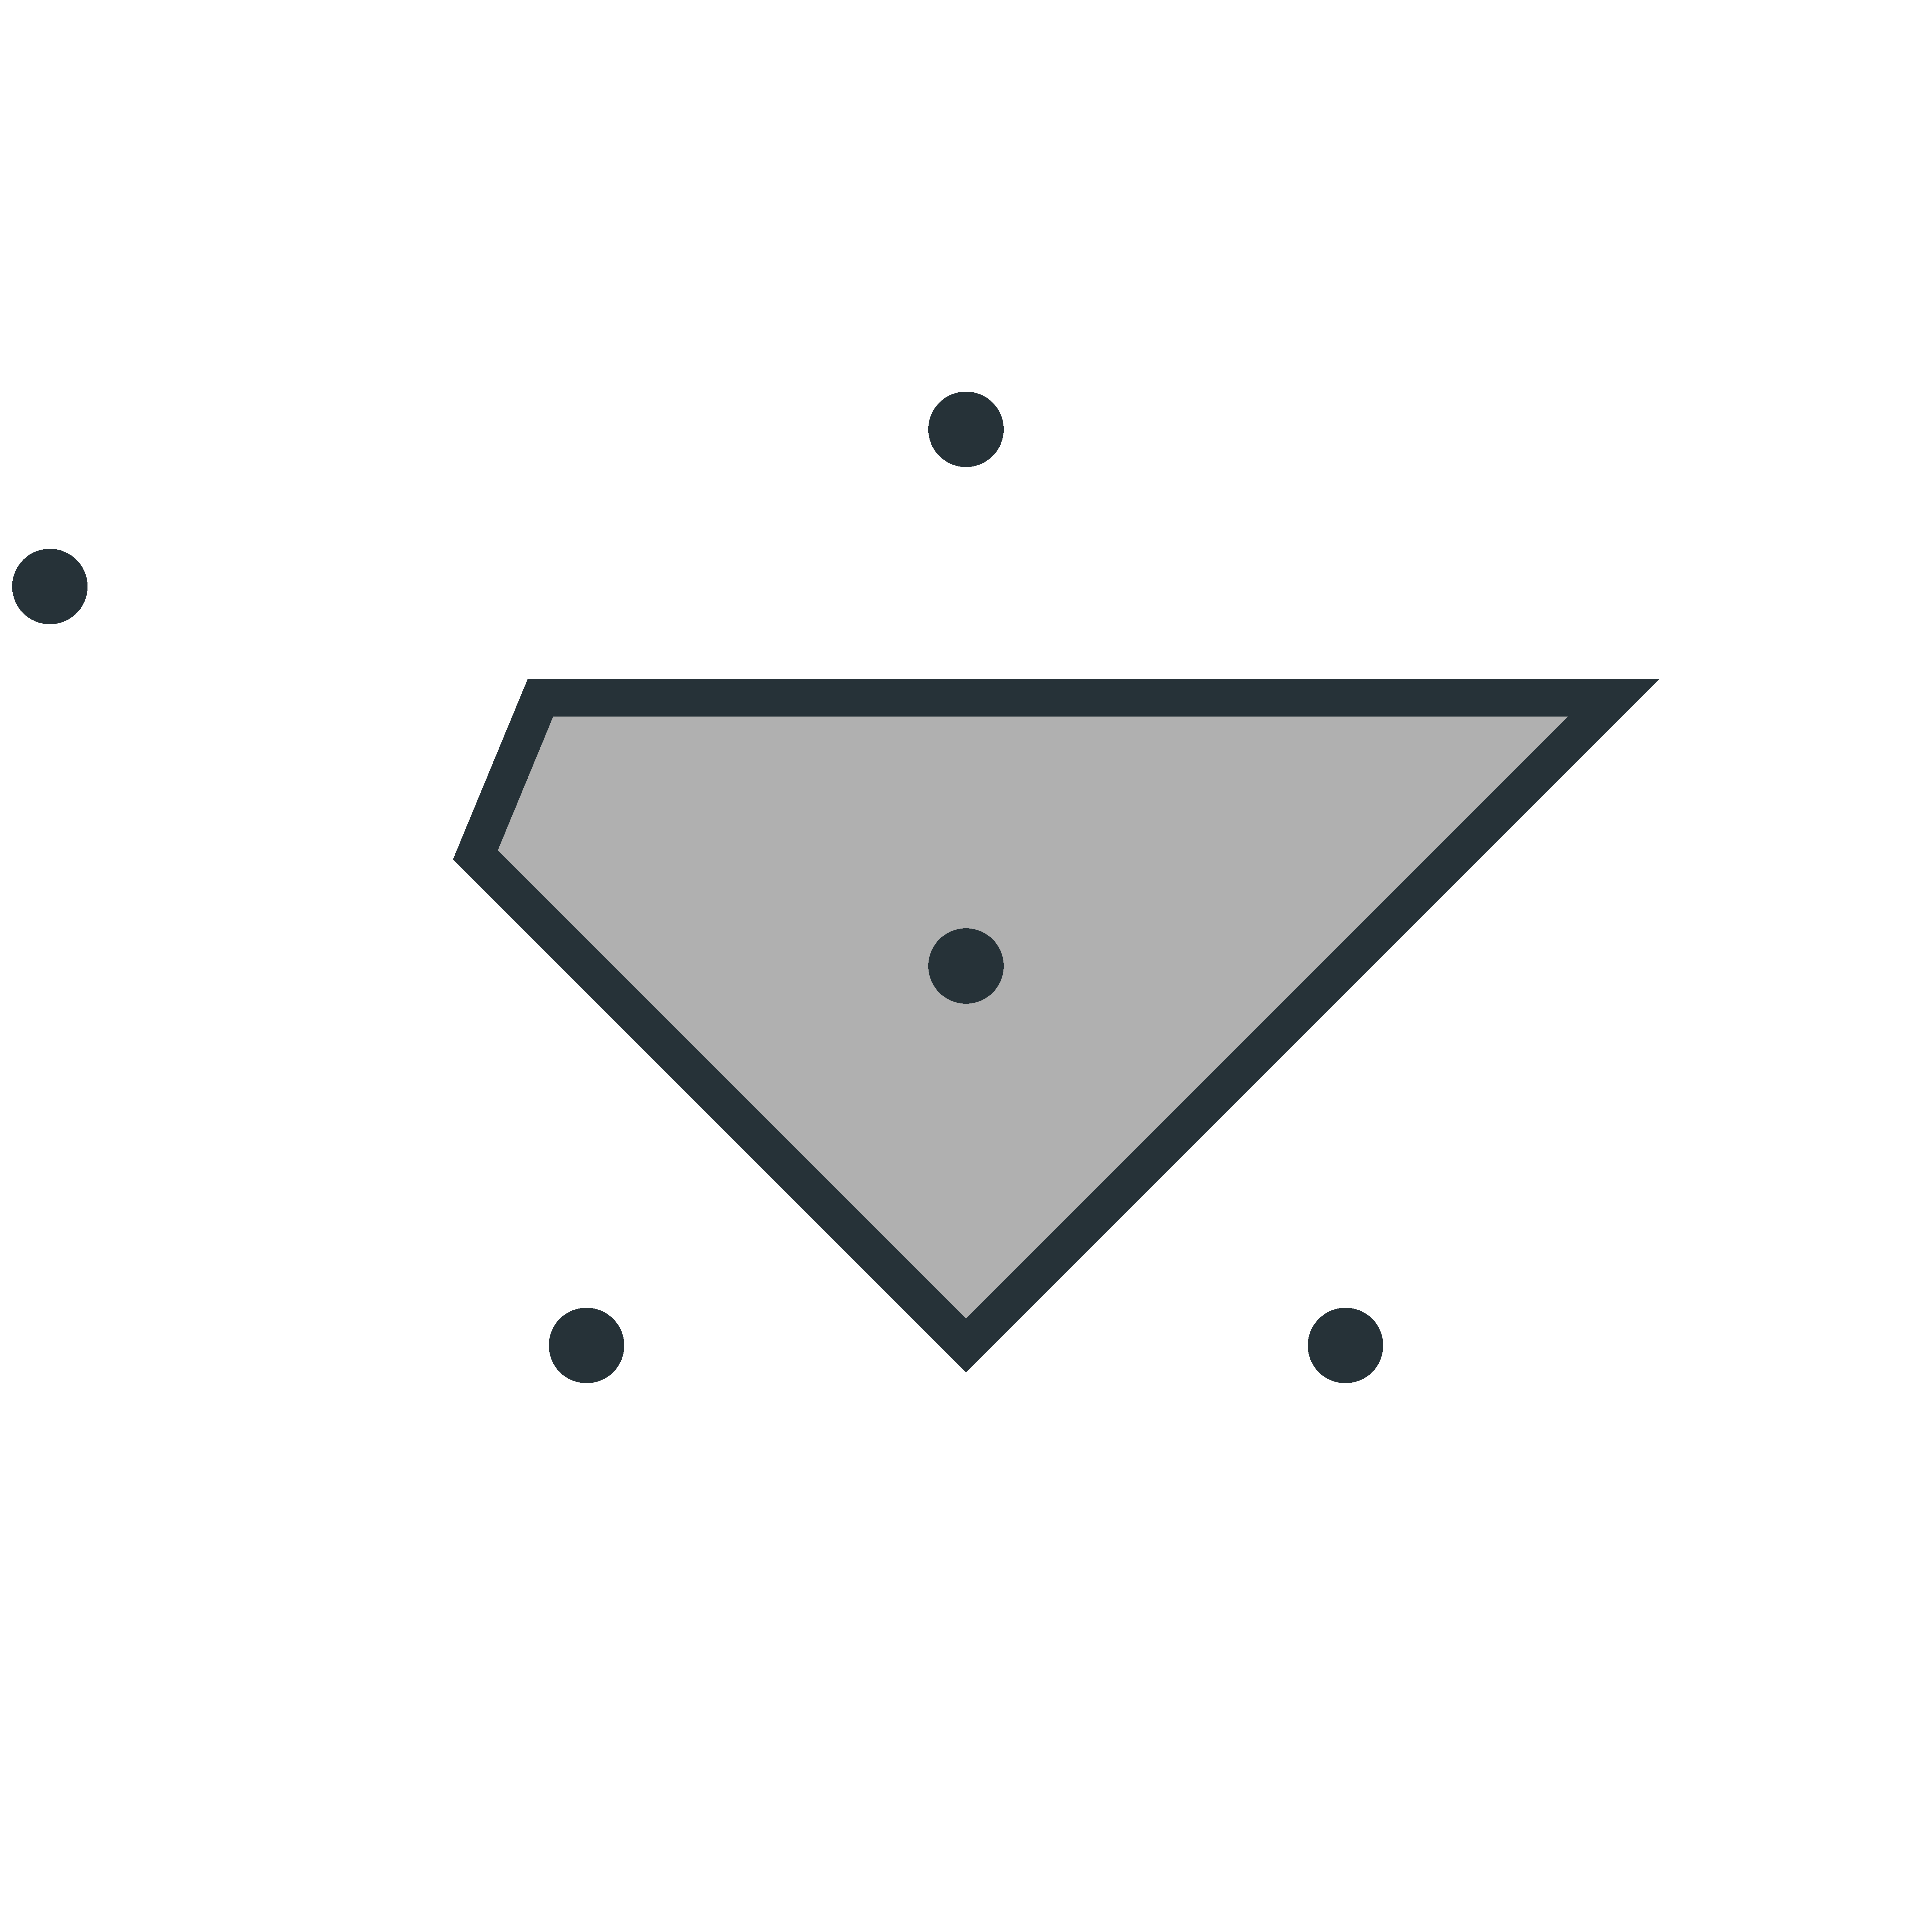
\includegraphics[width=0.11\textwidth]{img/results/tiles/octagon_100000_(1_0alpha_1)_028.pdf}
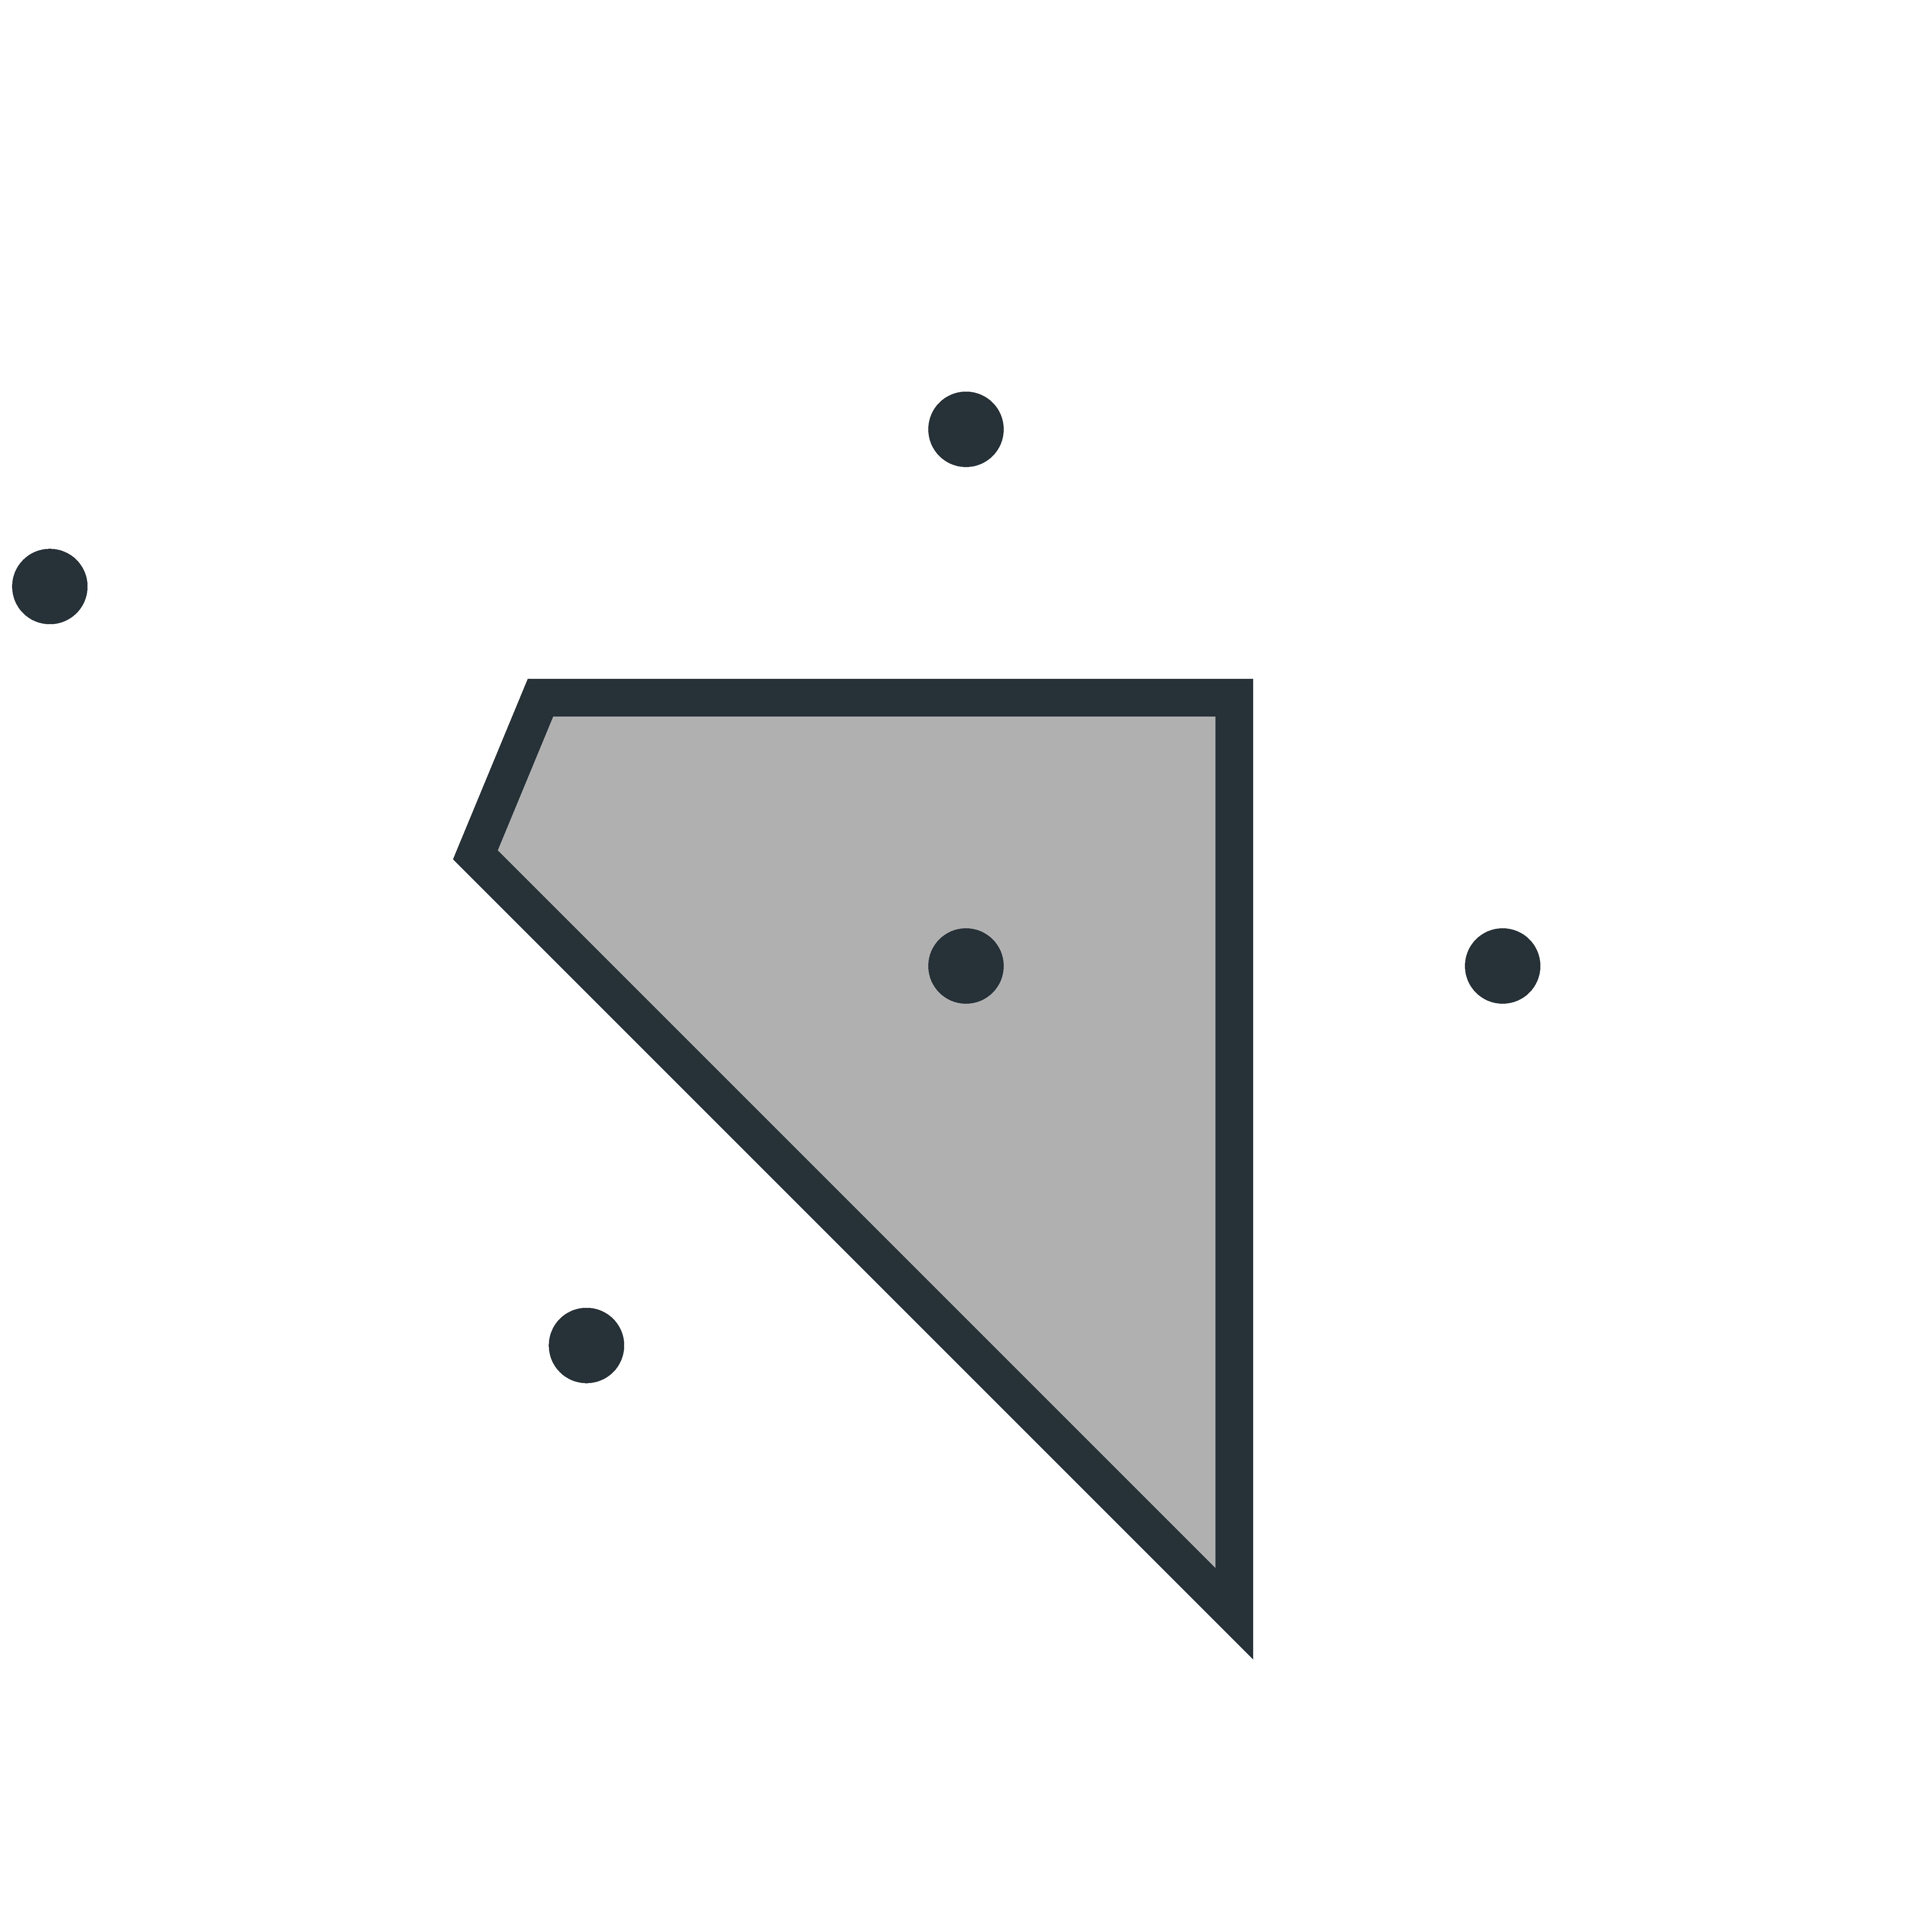
\includegraphics[width=0.11\textwidth]{img/results/tiles/octagon_100000_(1_0alpha_1)_029.pdf}
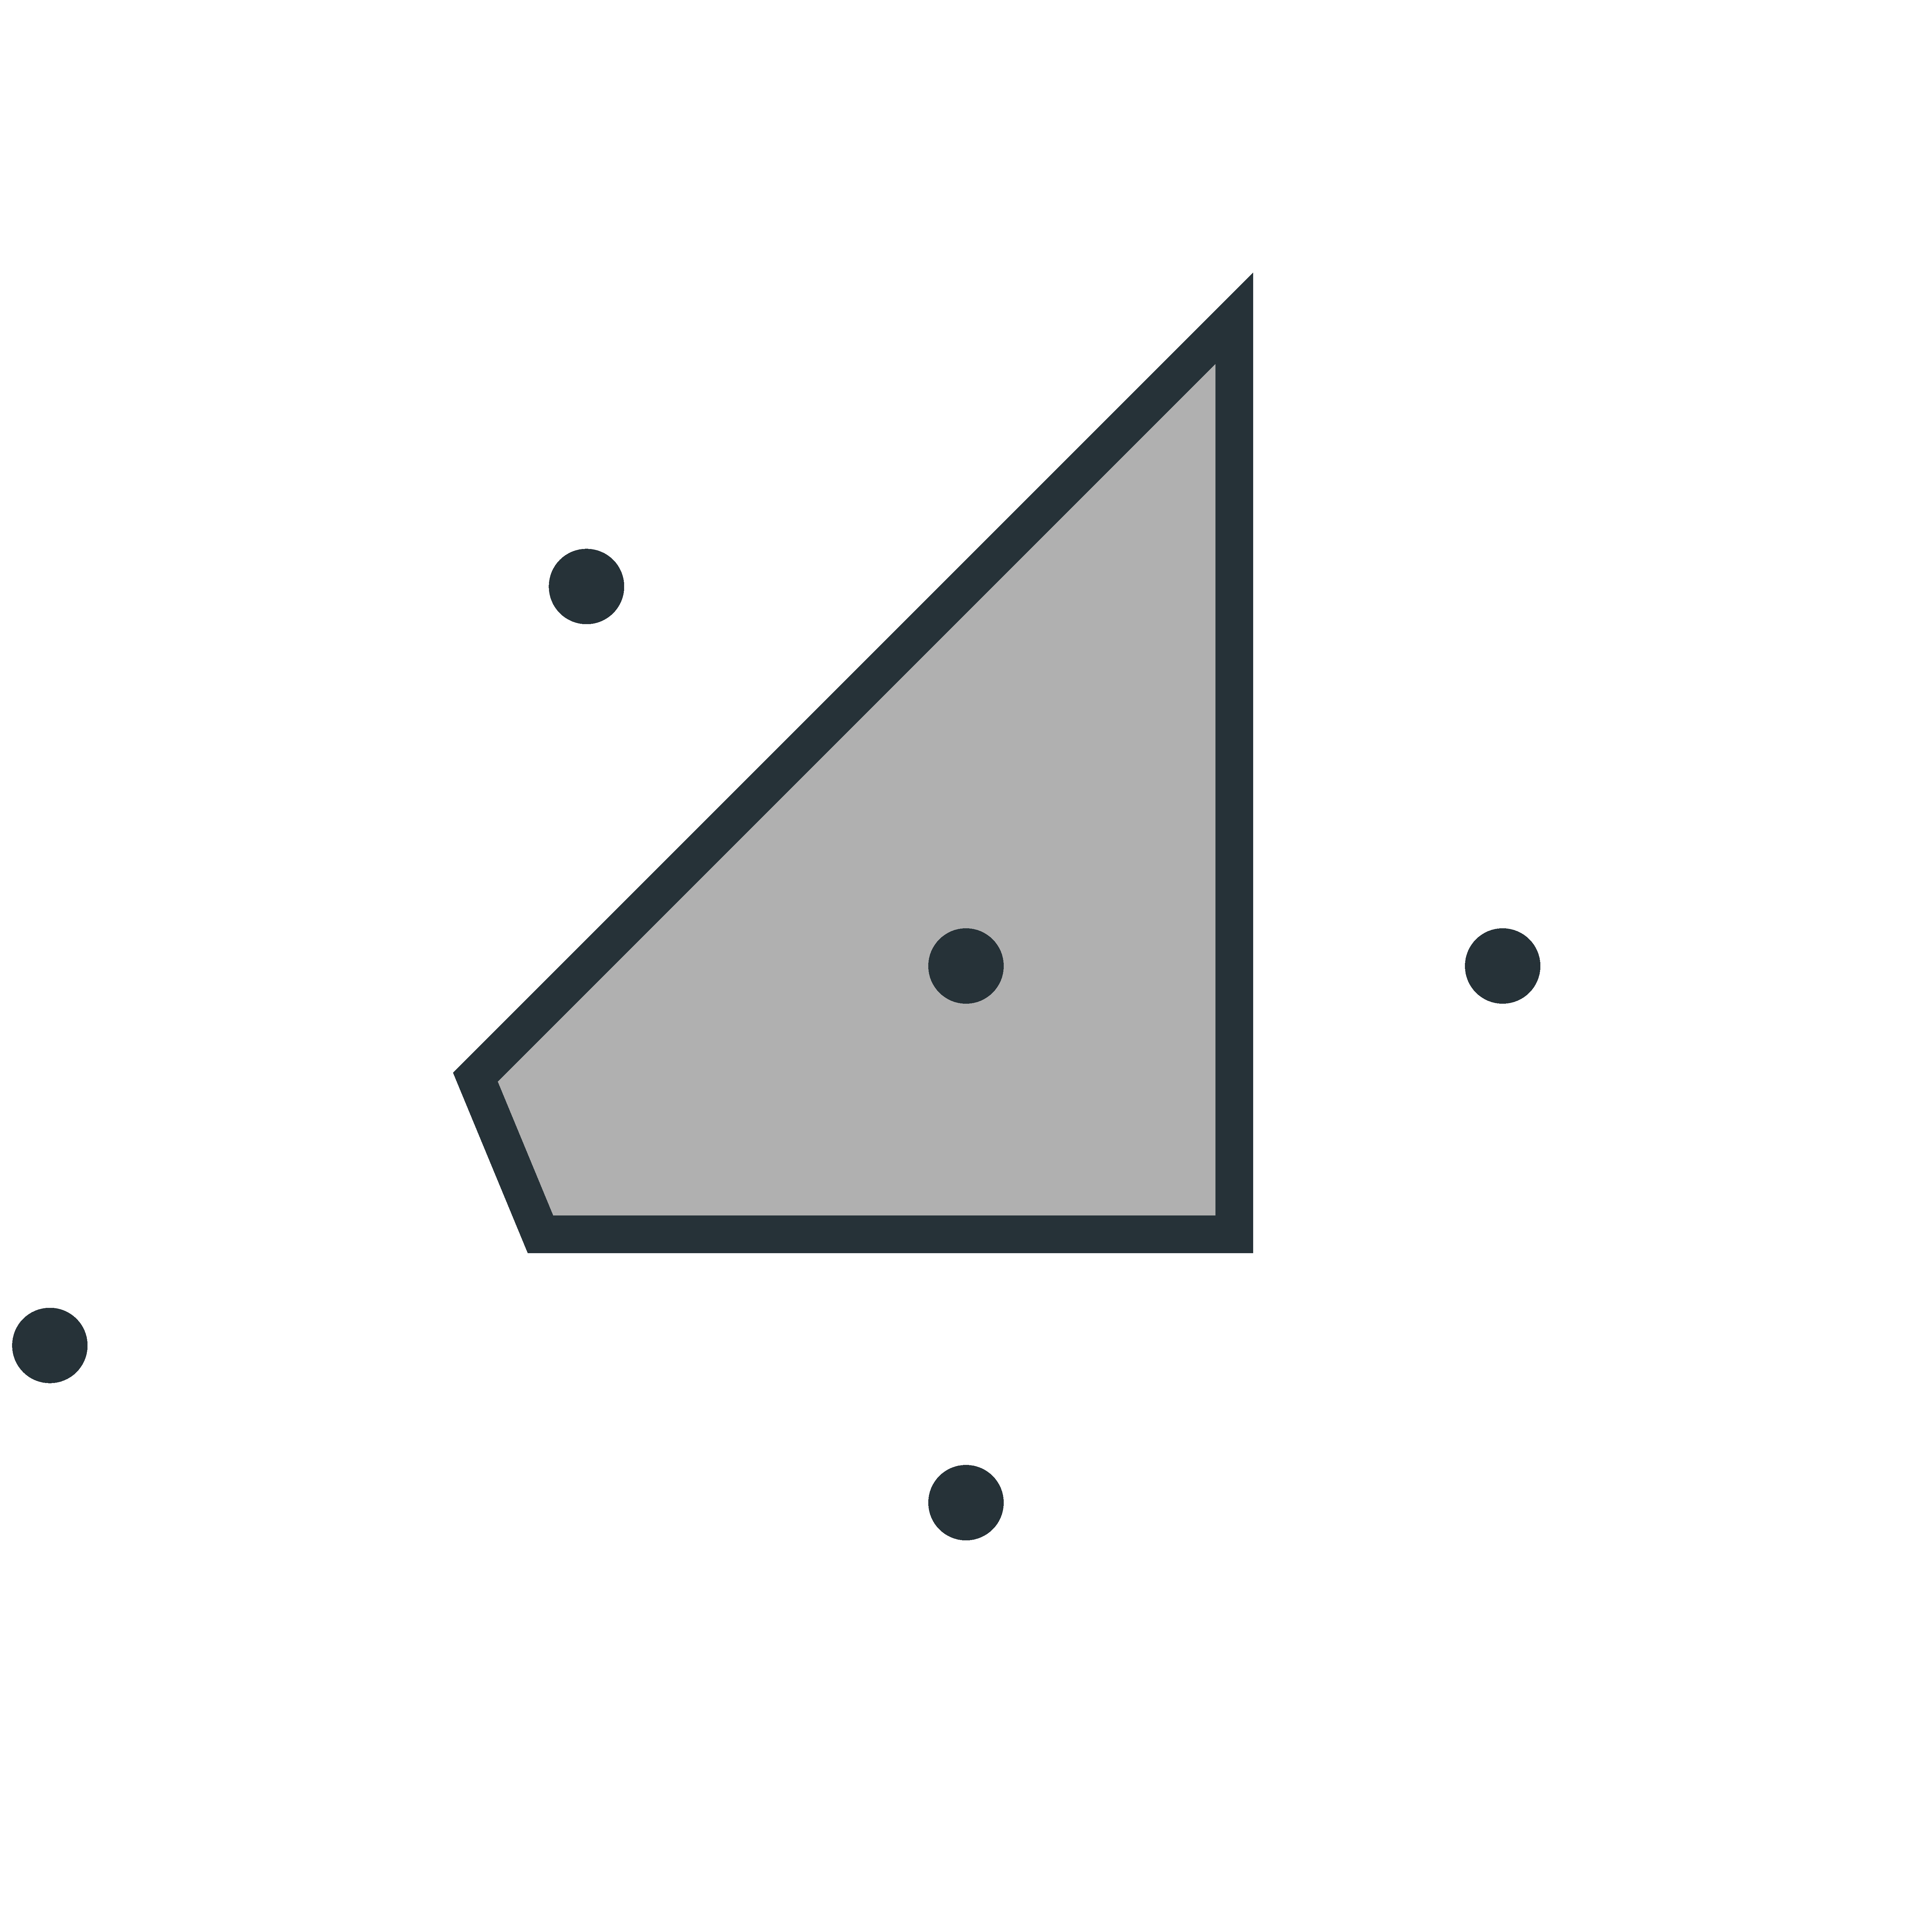
\includegraphics[width=0.11\textwidth]{img/results/tiles/octagon_100000_(1_0alpha_1)_030.pdf}
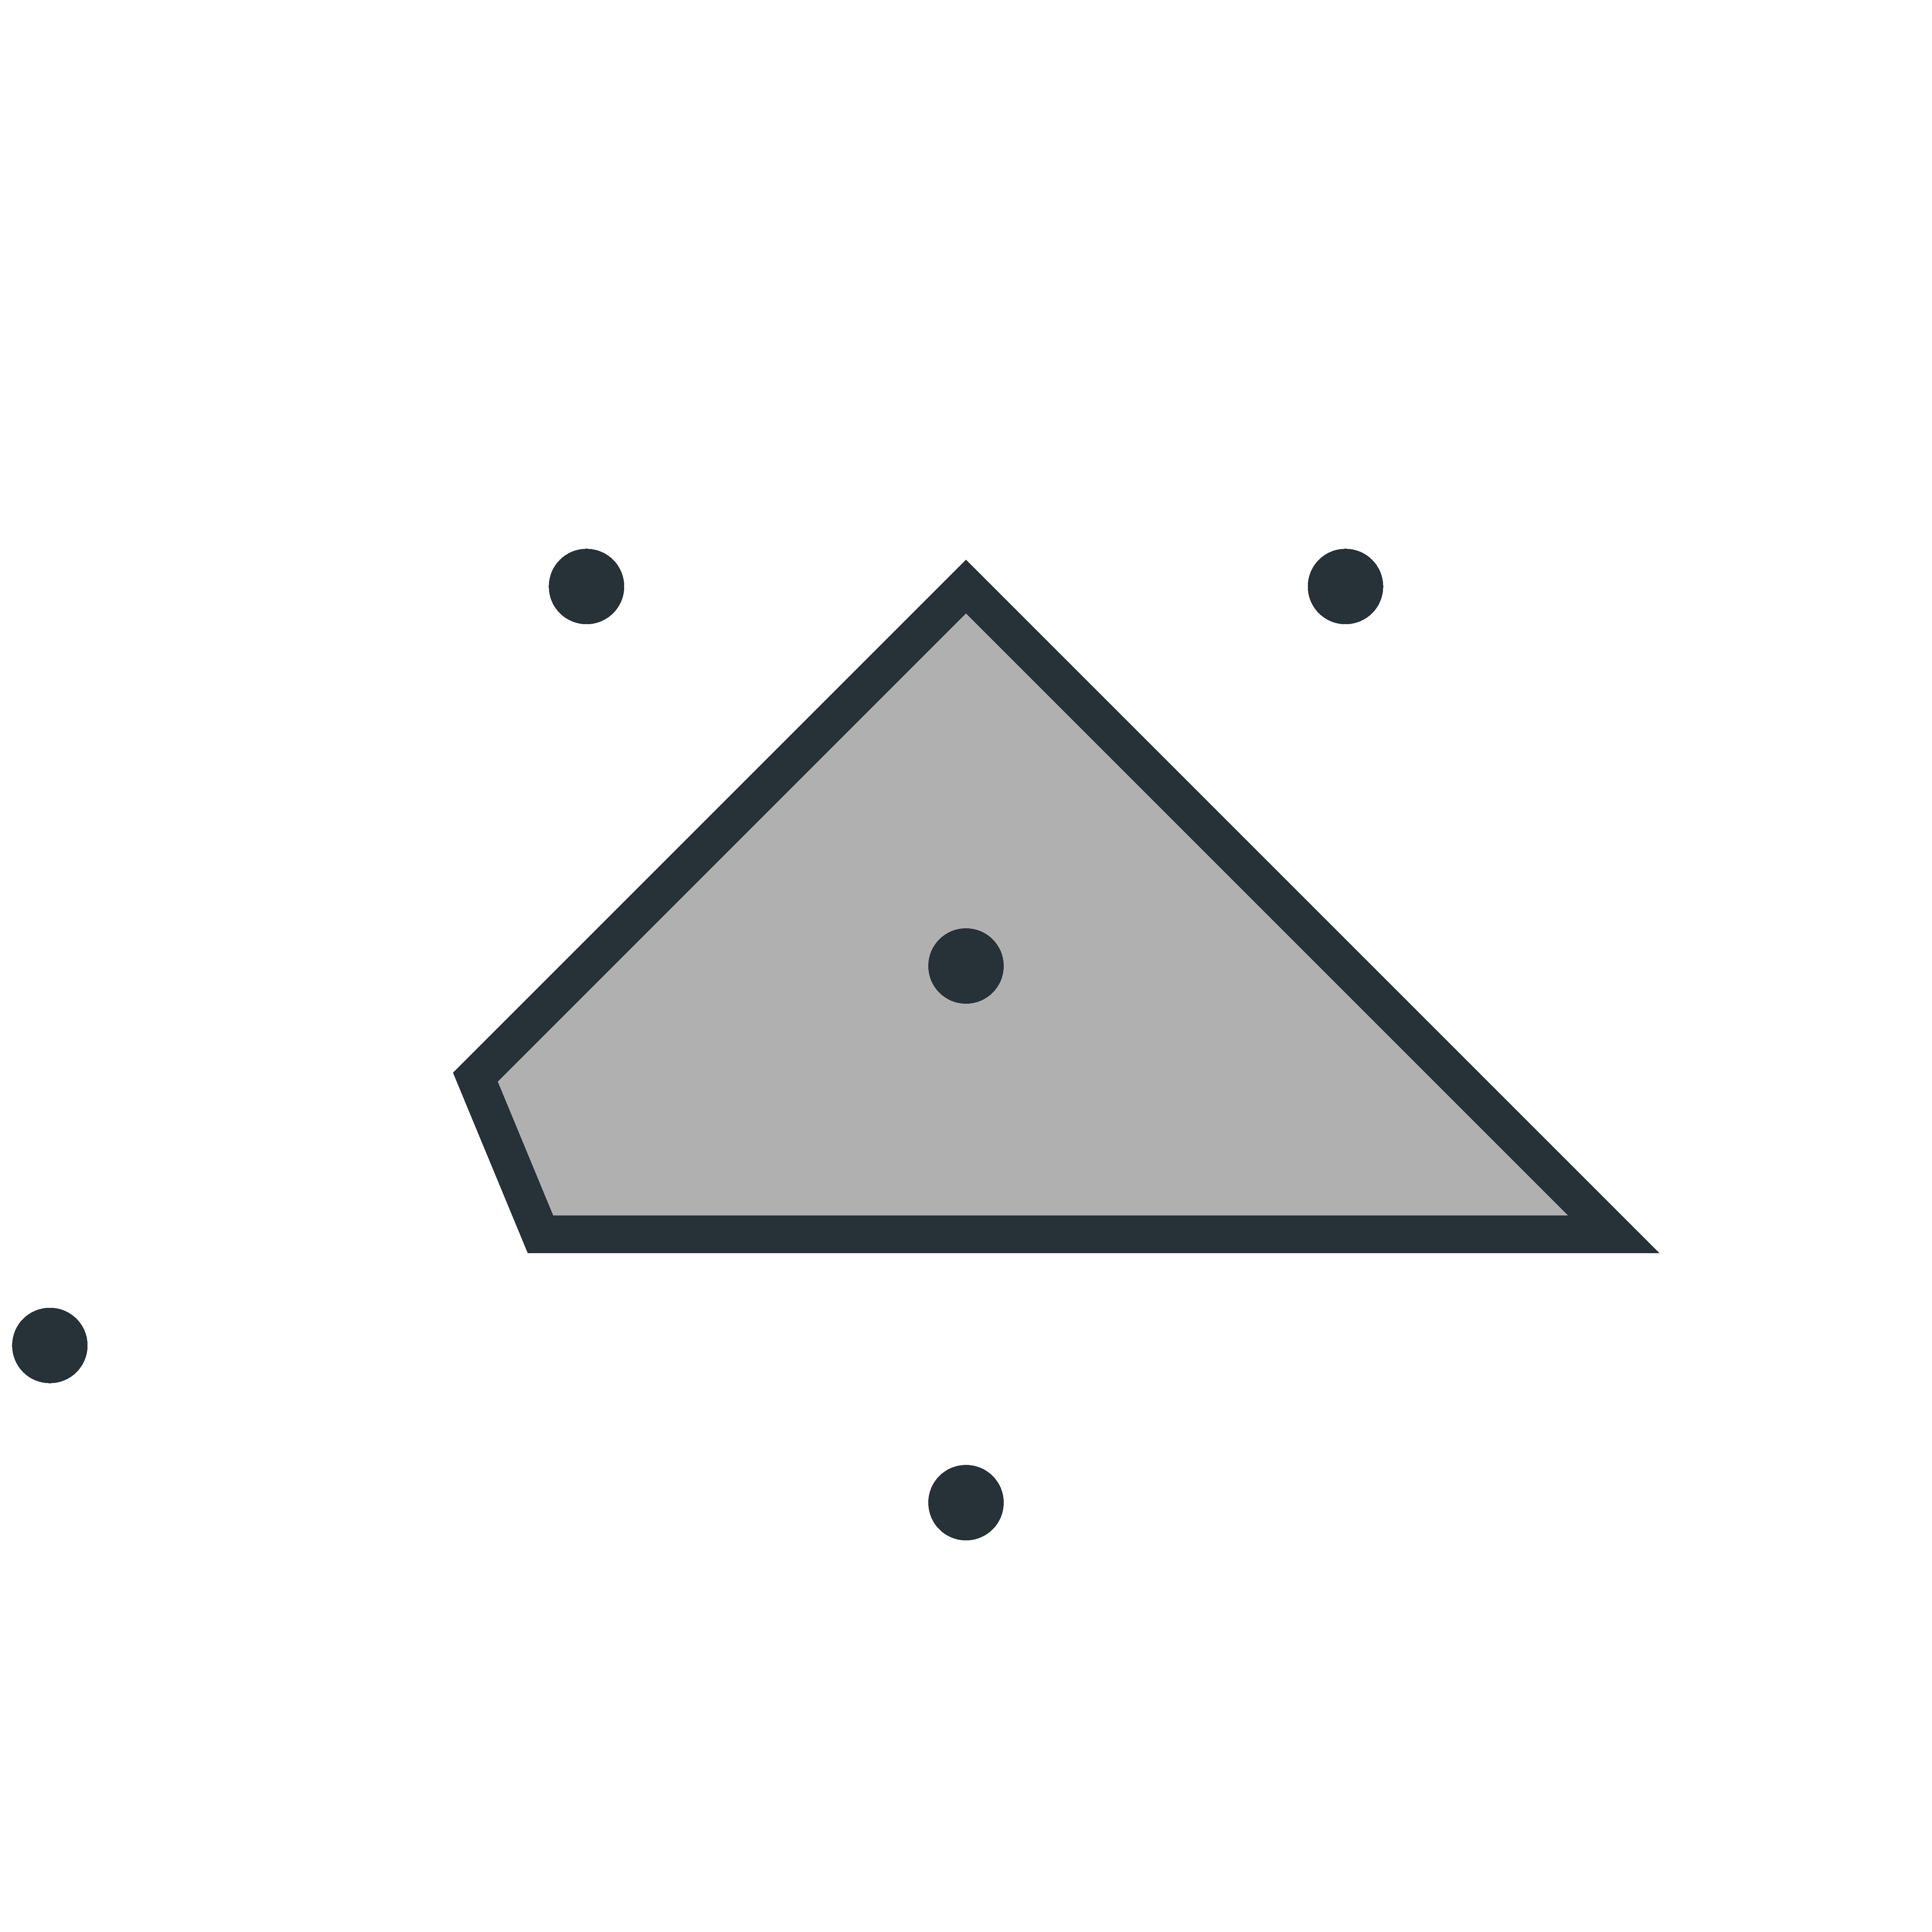
\includegraphics[width=0.11\textwidth]{img/results/tiles/octagon_100000_(1_0alpha_1)_031.pdf}
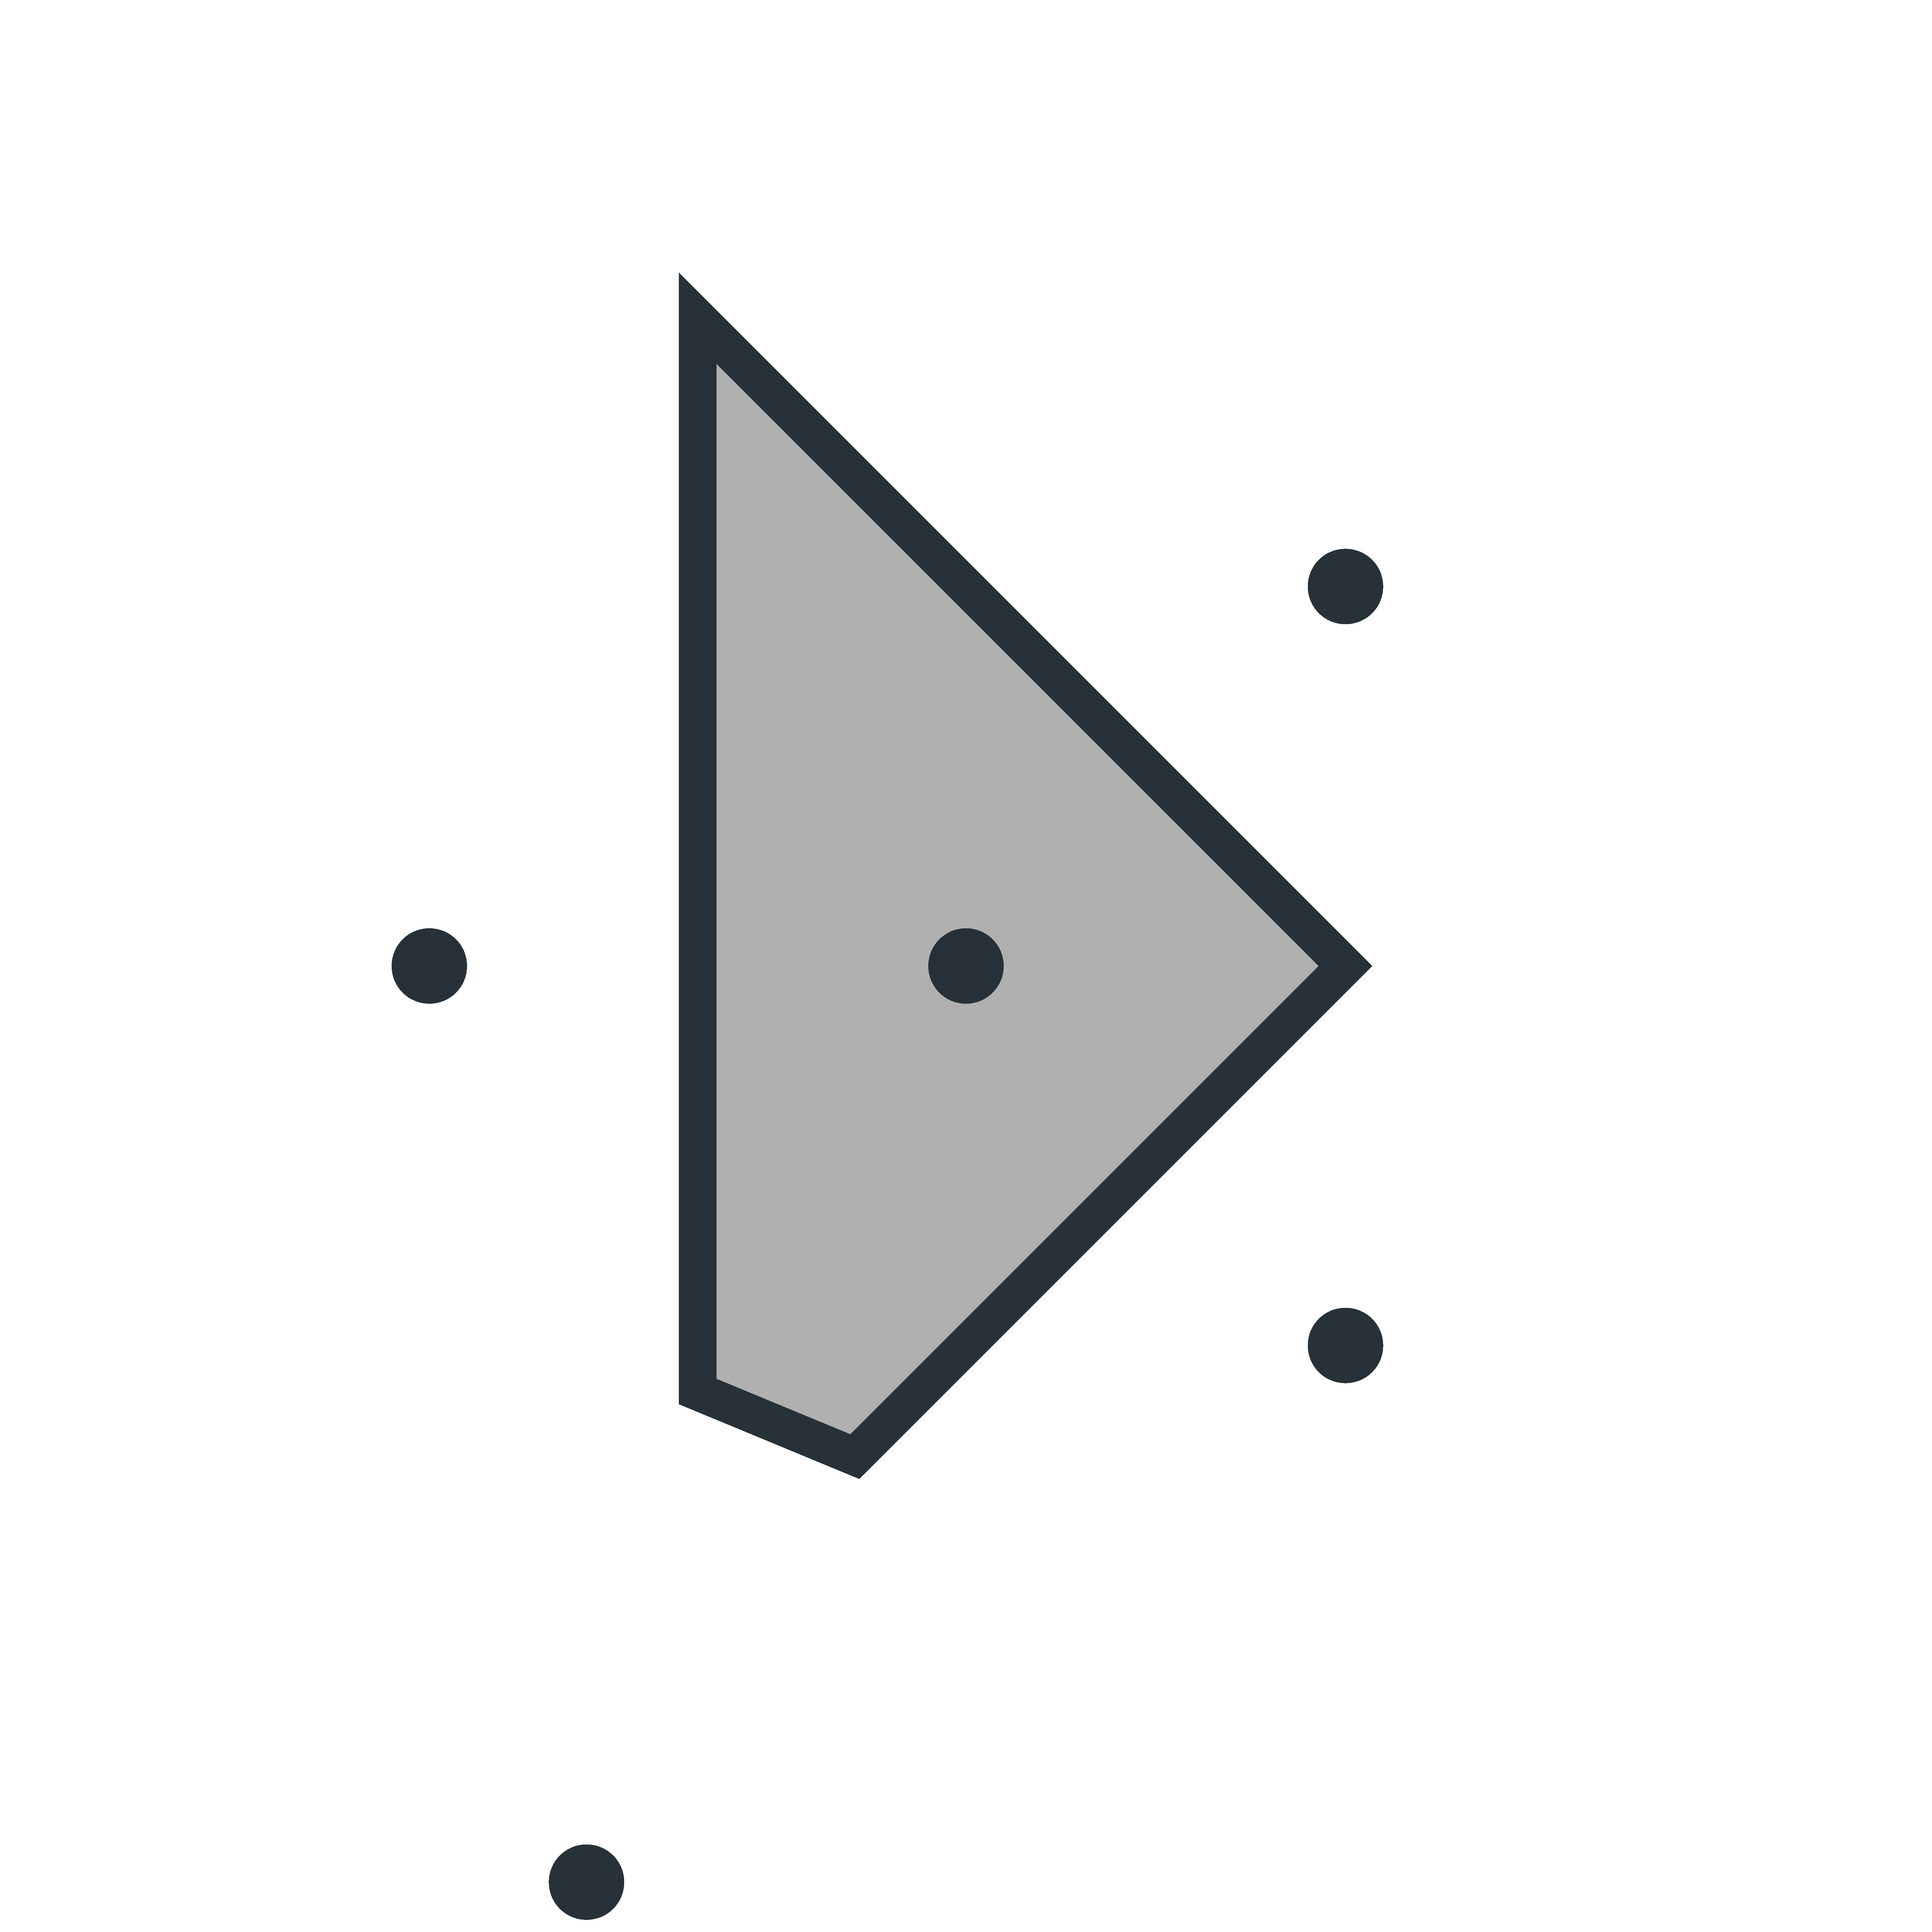
\includegraphics[width=0.11\textwidth]{img/results/tiles/octagon_100000_(1_0alpha_1)_032.pdf}

$\Downarrow$

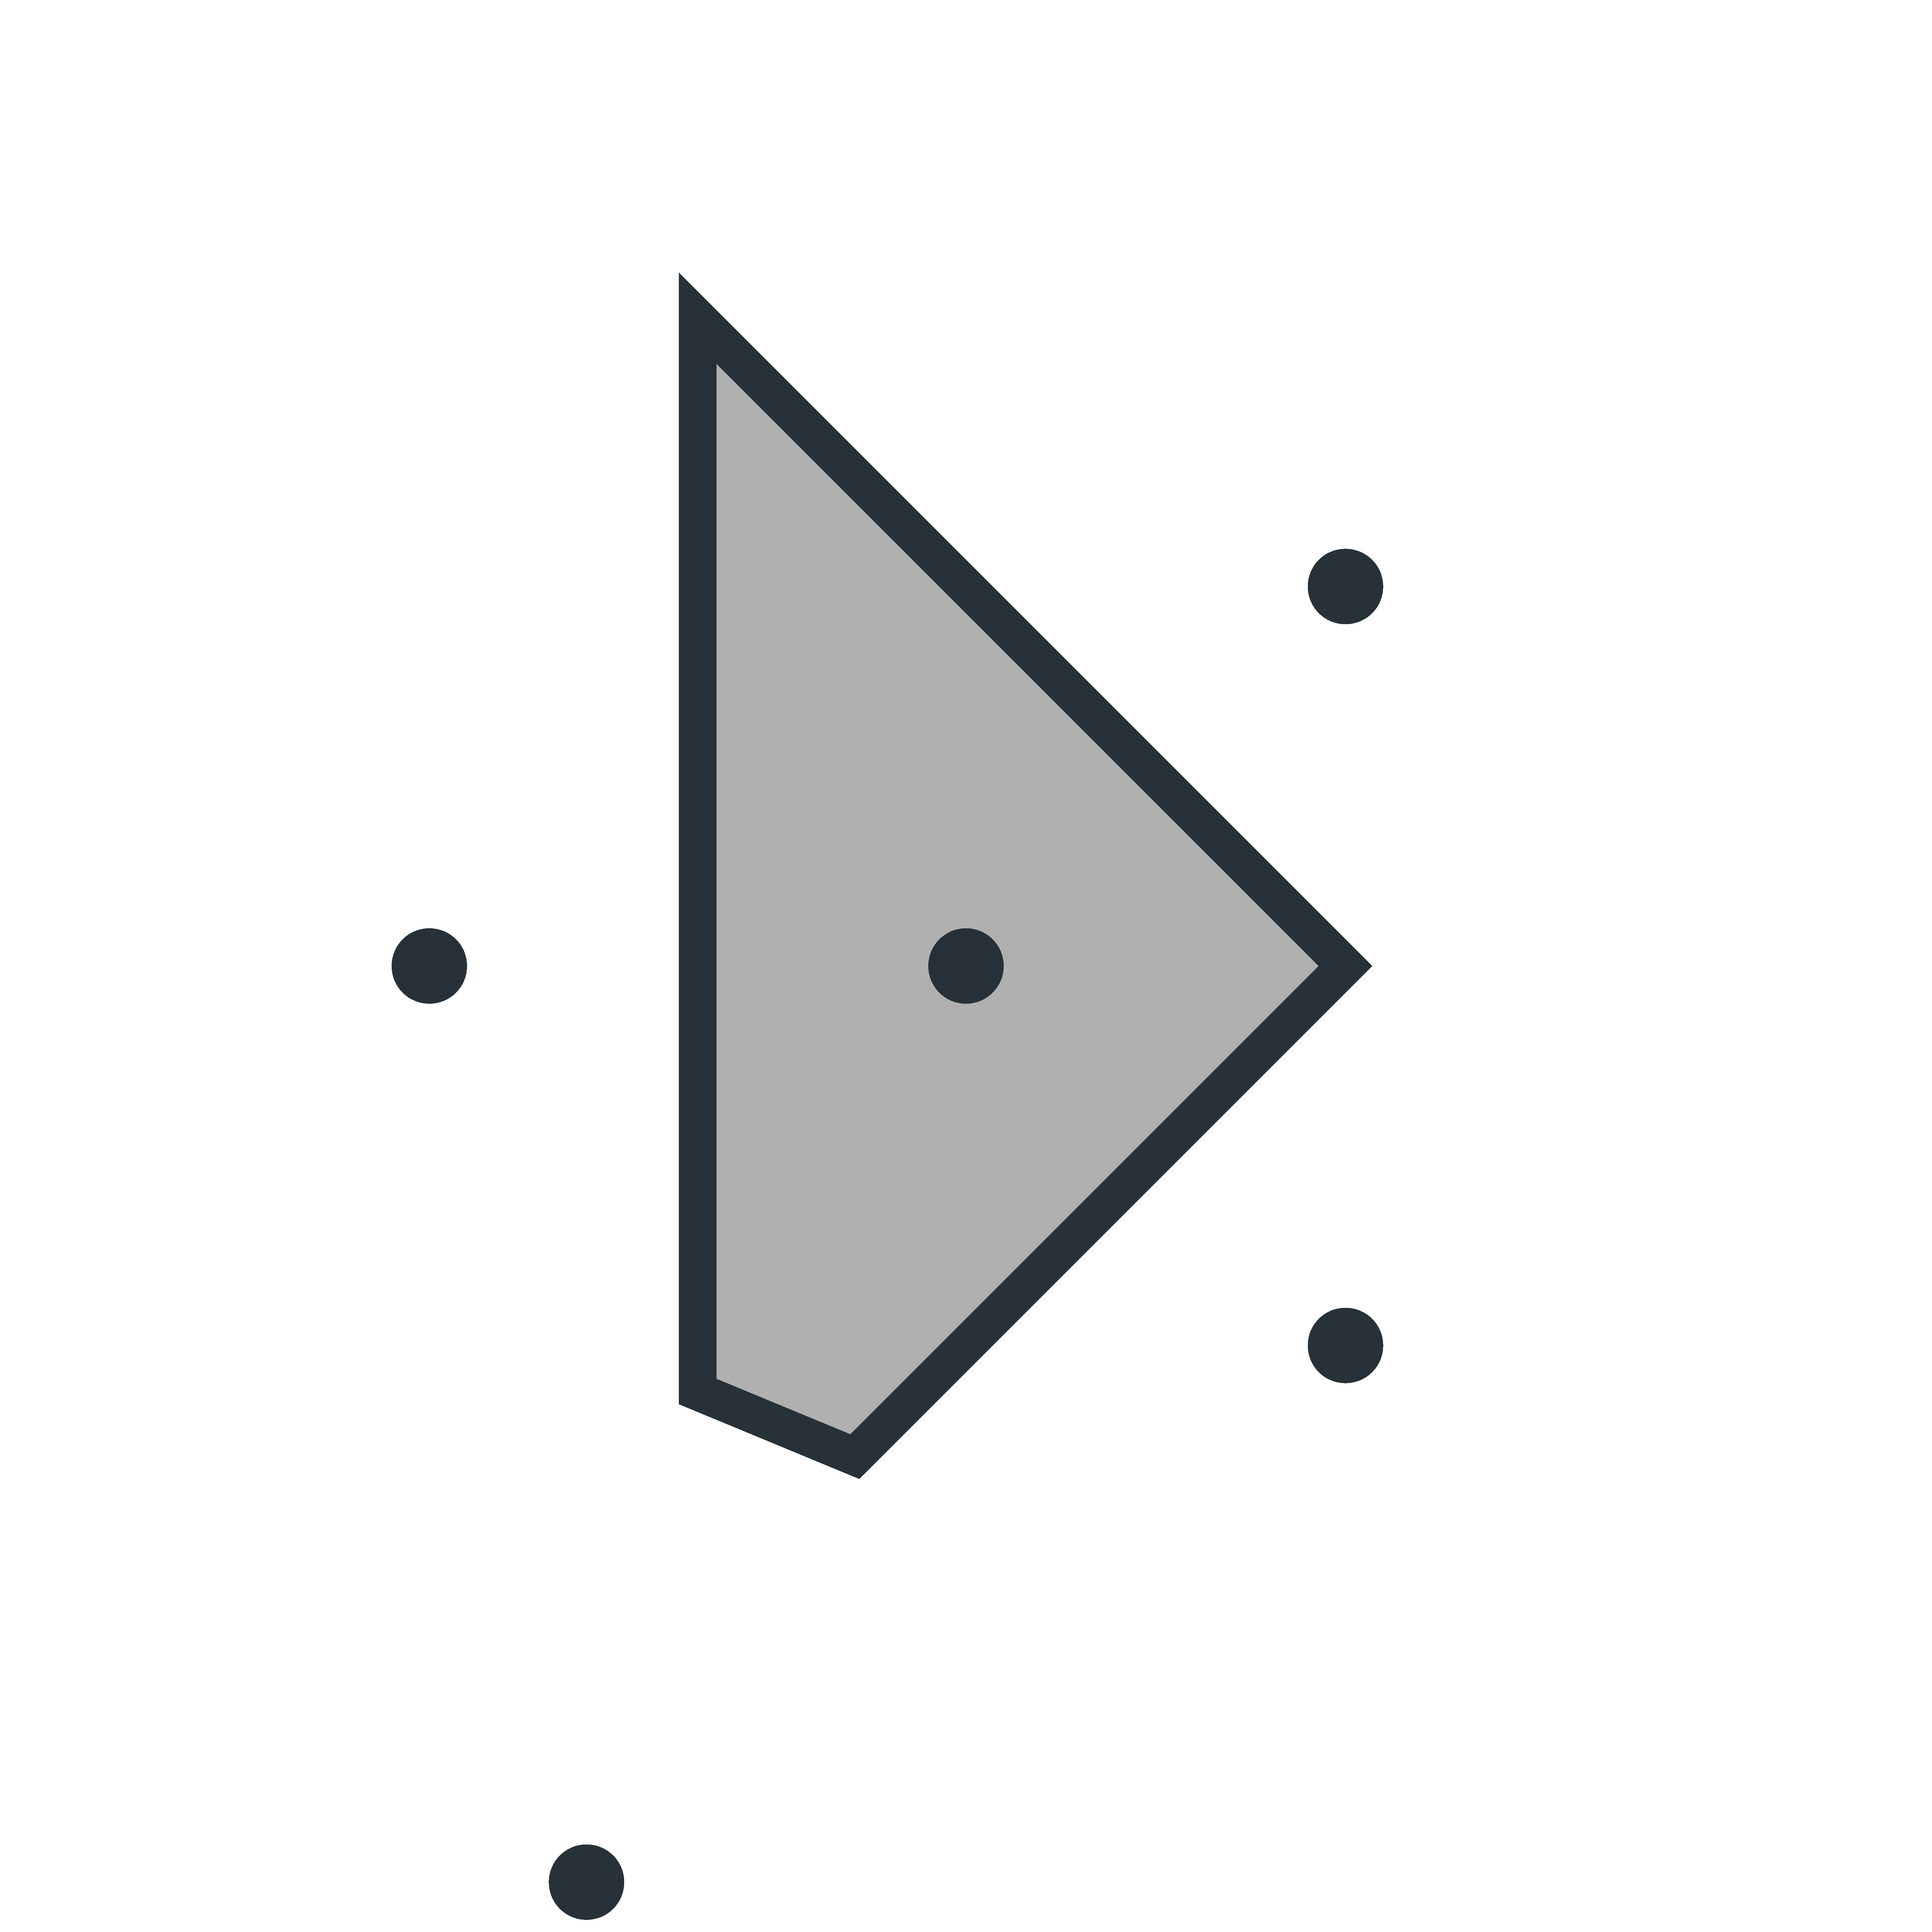
\includegraphics[width=0.11\textwidth]{img/results/tiles/octagon_100000_(1_0alpha_1)_pick.pdf}
\caption{Sixteen Voronoi tiles that have the same shape and appear in various orientations are all represented by one of them. }
\label{fig_results_tiles}
\end{figure}

The rows of Table \ref{tab_tiles1} correspond to window sizes: 
\begin{multicols}{2}
\begin{enumerate}
\item $1$
\item $\frac{5\beta_8-10}{2}$
\item $5\beta_8-11$
\item $\frac{13\beta_8-27}{4}$
\item $\frac{3\beta_8-5}{2}$
\item $\frac{4\beta_8-5}{4}$
\item $\frac{\beta_8}{2}$
\item $\frac{3\beta_8-2}{4}$
\item $\beta_8-1$
\item $\frac{2\beta_8+1}{4}$
\item $\frac{3}{2}$
\item $\frac{\beta_8+4}{4}$
\item $\frac{\beta_8+1}{2}$
\item $\frac{\beta_8+5}{4}$
\item $2$
\item $\frac{3\beta_8+1}{4}$
\item $\frac{3\beta_8-3}{2}$
\item $\frac{4\beta_8-1}{4}$
\item $\frac{\beta_8+2}{2}$
\item $\frac{7\beta_8-8}{4}$
\item $3\beta_8-5$
\item $\frac{5\beta_8-3}{4}$
\item $\frac{7-\beta_8}{2}$
\item $\frac{\beta_8+7}{4}$
\item $\beta_8$
\end{enumerate}
\end{multicols}

The columns of Table \ref{tab_tiles1} correspond to the Voronoi tiles from Figure \ref{fig_tiles1}. 

\end{document}
